%\chapter{Détection de sections et entités juridiques}
\chapter{Annotation des sections et entités juridiques}
\label{chap:structuration}

% court abstract
% Objectif: L'annotation manuelle peut atteirndre des interagréments raisonables (kappa) et nous démontrons qu'il est faisable d'automatiquement annoter les sections et métadonnées de référence d'un jugement à l'aide de modèle probabiliste graphiques comme le CRF ou le HMM moyennant de bien choisir les features
%Mots clés: annotation d'entités nommées judiciaires, chaine caché de markov, champ conditionnel aléatoires

\textit{\small \textbf{Résumé.} Ce chapitre traite de la détection de sections et des mentions (occurrences) d'entités dans les décisions de justices françaises. Ce problème est important car il vise une structuration des documents par le balisage des sections organisant le document, des méta-données de référence de l'affaire, et des citations des normes juridiques employées. Cette annotation automatique facilite la lecture des décisions et fournit des méta-données pour rapidement indexer et retrouver des  décisions. Le problème est formulée en des tâches d'étiquetage de séquence puisque tout document textuel est une séquence de mots, de lignes, etc. Les principales contributions discutées ici sont : l'annotation manuelle d'un corpus d'évaluation de 500 documents, une analyse de l'application des modèles probabilistes graphiques HMM et CRF, et des discussions sur l'impact de divers aspects de la conception d'un système d'annotation par étiquetage de séquence. Les expérimentations effectuées permettent de comparer l'ingénierie manuelle et l'ingénierie automatique de la représentation des objets à classer, de comparer des schéma d'étiquetage, d'analyser l'effet de l'augmentation des données d'entrainement sur la qualité des annotations. Les résultats montrent principalement l'efficacité des modèles à base de champs aléatoires conditionnels à chaîne linéaire (CRF) pour les différentes tâches.}


\section{Introduction}
\label{sec:structuration:motivation}

Bien que les décisions ne soient pas structurées, leur contenu est organisé en sections dont les principales sont: l'entête, le corps, et le dispositif. Chacune de ces sections décrit des informations spécifiques de l'affaire: 
\begin{itemize}
	\item l'entête contient de nombreuses méta-données de référence comme la date, le lieu, les participants, etc.
	\item le corps détaille les faits, les procédures antérieures, les conclusions des parties et le raisonnement des juges ;
	\item le dispositif est la synthèse du résultat final c'est-à-dire qu'on y retrouve les réponses aux demandes des parties.
\end{itemize}

Certaines informations spécifiques se retrouvent très souvent dans une même section, e.g. méta-données (localisation, date), prétentions des parties, décisions finales. Compte tenu de la répartition standard de certaines informations, certaines tâches d'extraction d'information peuvent être abordées comme des traitements spécifiques à appliquer à certaines sections. Ce chapitre traite dans un premier temps des modèles utilisés pour appliquer cette phase de segmentation des décisions en sections. Par la suite, les entités, et données sur les demandes et résultats, pourront plus facilement être extraites. Nous nous focaliserons en particulier ici sur la détection des mentions d'entités telles que la date à laquelle le jugement a été prononcé, le type de juridiction, sa localisation (ville), les noms des juges, des parties, et les règles de loi citées (normes). La Table \ref{tab:structuration:relevantinfo} liste les différentes entités cibles et fournit des exemples illustrant leurs occurrences dans les décisions avec lesquelles nous avons travaillé.

\begin{table}[!ht]
\scriptsize
\begin{tabular}[c]{|p{0.17\textwidth}|c|p{0.37\textwidth}|cc|}
\hline
\textbf{Entités} & \textbf{Label} & \textbf{Exemples} & \multicolumn{2}{c|}{\textbf{\#mentions}$^a$}\\
  & & & \textbf{Médiane}$^b$& \textbf{Total}$^c$ \\ \hline
Numéro de registre général (R.G.) & \textbf{rg} & \og 10/02324 \fg{}, \og 60/JAF/09 \fg{} & 3 & 1318\\ \hline
Ville & \textbf{ville}& \og NÎMES \fg{}, \og Agen \fg{}, \og Toulouse \fg{} & 3 & 1304\\ \hline
Juridiction & \textbf{juridiction} & \og COUR D'APPEL \fg{} & 3 & 1308\\ \hline
Formation & \textbf{formation} &  \og 1re chambre \fg{}, \og Chambre économique \fg{} & 2 &  1245\\ \hline
Date de prononcé & \textbf{date} & \og 01 MARS 2012 \fg{}, \og 15/04/2014 \fg{} & 3 & 1590\\ \hline
Appelant & \textbf{appelant} & \og SARL K. \fg{}, \og Syndicat ... \fg{}, \og Mme X ... \fg{} & 2 & 1336 \\ \hline
Intimé & \textbf{intime} & - // - & 3 & 1933 \\ \hline
Intervenant & \textbf{intervenant} & - // - & 0 & 51 \\ \hline
Avocat & \textbf{avocat} & \og Me Dominique A., avocat au barreau de Papeete \fg{} & 3 & 2313\\ \hline
Juge & \textbf{juge} & \og Monsieur André R. \fg{}, \og Mme BOUSQUEL \fg{} & 4 & 2089\\ \hline
Fonction de juge & \textbf{fonction} & \og Conseiller \fg{}, \og Président \fg{} & 4 & 2062\\ \hline
Norme & \textbf{norme} & \og l' article 700 NCPC \fg{}, \og articles 901 et 903 \fg{} & 12 & 7641 \\ \hline
%Argent & \textbf{argent} & "un euro", "" & 14$^*$ & 1777$^*$ \\ \hline
\noalign{\smallskip}\hline\noalign{\smallskip}
Non-entité & \textbf{O} & \textit{mot ne faisant partie d'aucune mention d'entité} & - & -\\ \hline
\end{tabular} 

$^a$ nombre de mentions d'entités dans le corpus annoté pour les expérimentations

$^b$ nombre médian de mentions par document dans le corpus annoté

$^c$ nombre total d'occurrences dans le corpus annoté

$^*$ Les statistiques sur les sommes d'argent ne concernent que 100 documents annotés (max=106, min=1, moyenne=17.77), contre 500 documents pour les autres entités.

\caption{Exemples d'entités et statistiques sur la base d'exemples annotés manuellement }\label{tab:structuration:relevantinfo}
\end{table}

On pourrait s'attendre à ce qu'une institution comme la justice respecte un modèle strict et commun à tous les tribunaux pour la rédaction des décisions pour permettre de facilement pouvoir les lire et les analyser. Malheureusement, même si les  décisions décrivent des informations de même nature, le modèle employé semble varier entre les juridictions. C'est ce que l'on remarque déjà au niveau de la transition entre sections. Au vu de leur rôle, il est évident que les sections devraient être séparées par des marqueurs bien précis. Une approche intuitive de sectionnement consisterait par conséquent à définir un algorithme capable de reconnaître automatiquement ces marqueurs de transition par l'utilisation d'expressions régulières. Cependant, les marqueurs retrouvés ne sont généralement pas standards. Les indicateurs de transitions sont en effet souvent différents d'une décision à l'autre ; ils peuvent correspondre à des titres ou des motifs à base de symboles (astérisques, tirets, etc.). Il arrive même parfois que la transition soit implicite et que l'on ne s'en rende compte que par la forme ou le contenu des lignes, au cours de la lecture. Même les marqueurs explicites sont hétérogènes. Lors de l'emploi de titres par exemple, la transition de l'entête à l'exposé du litige peut être indiquée par des titres comme \og {Exposé} \fg{}, \og {FAITS ET PROCÉDURES} \fg{}, \og {Exposé de l'affaire} \fg{}, \og {Exposé des faits} \fg{}, etc. Quant au dispositif, il est introduit généralement par l'expression \og {PAR CES MOTIFS} \fg{} avec souvent quelques variantes qui peuvent être très simples (par exemple \og {Par Ces Motifs} \fg{}) ou exceptionnelles (par exemple \og {P A R C E S M O T I F S :} \fg{}). Dans certaines décisions, cette expression est remplacée par d'autres expressions comme \og {DECISION} \fg{}, \og {DISPOSITIF} \fg{}, \og {LA COUR} \fg{}, etc. 
Par ailleurs, lors de l'utilisation de symboles, il arrive qu'un même motif sépare différentes sections et même des paragraphes dans une même section. Des différences similaires apparaissent aussi pour les entités. Les noms de parties sont généralement placés après un mot particulier comme  \og {APPELANTS} \fg{} ou \og {DEMANDEUR} \fg{} pour les demandeurs (appelants en juridiction de 2e degré), \og {INTIMES} \fg{} ou \og {DEFENDEUR} \fg{} pour les défendeurs (ou intimés), et  \og {INTERVENANTS} \fg{} pour les intervenants. Les noms des individus, sociétés et lieux commencent par une lettre majuscule, et sont entièrement en majuscules. Cependant, certains mots communs peuvent apparaître aussi en majuscules (par ex. {APPELANTS}, {DÉBATS}, {ORDONNANCE DE CLÔTURE}). Les entités peuvent contenir des chiffres (identifiants, dates, ...), des caractères spéciaux ( \og / \fg{},  \og - \fg{}), des initiales (par ex. \og A. \fg) ou abréviations.  Dans l'entête, les entités apparaissent généralement dans le même ordre (par ex. les appelants avant les intimés, les intimés avant les intervenants). Cependant, on rencontre une multitude de types d'entités dans l'entête, contrairement aux autres sections où seules les normes nous intéressent. De plus, le texte est mieux structuré dans l'entête que dans les autres sections. Ces nombreuses différences entre décisions rendent inadéquates les expressions régulières.

Notre étude consiste à analyser l'application du Modèle Caché de Markov (HMM) et des Champs Aléatoires Conditionnels (CRF) aux problèmes de sectionnement et reconnaissance d'entités juridiques. Ces deux tâches sont ainsi représentées sous la forme d'un problème d'étiquetage de séquences. L'idée est de découper un texte en segments atomiques distincts (\textit{token}) qui peuvent être des mots, des phrases, des paragraphes, etc. Le texte est ainsi représenté sous forme de séquences et chaque objet d'intérêt (section ou entité) comprend  un ou plusieurs segments. Un label est défini pour chaque type d'entité (par ex. \verb|PER| pour les noms de personnes). 


\section{Extraction d'information par étiquetage de séquence}
\label{sec:structuration:biblio}

Parmi les approches d'extraction d'information \citet{chau2002nerwithNN}, on retrouve principalement :

\begin{itemize}
\item Les \textbf{systèmes à recherche lexicale} sont conçus sur la base d'une liste d'entités préalablement connues, et leurs synonymes dans le domaine d'intérêt. Par exemple, dans le domaine juridique, un lexique pourrait contenir les identifiants de règles juridiques et les noms des juges. La liste des entités peut être fournie par des experts ou apprise à partir d'un ensemble de données annotées manuellement (phase d'apprentissage). Cependant, il s'avère très difficile de maintenir une telle liste car le domaine change régulièrement (nouvelles lois par ex.). De plus, les mentions d'entités peuvent avoir plusieurs variantes. Par exemple, la même règle juridique \og Article 700 du code de procédure civile \fg{} peut être citée seule et en entier (\og article 700 du code de procédure civile \fg{}), ou abrégée (\og article 700 CPC \fg{}), ou encore avec d'autres règles (\og articles 700 et 699 du code de procédure civile \fg{}). De plus, ces approches sont sujettes aux problèmes d'ambiguïté, par exemple lorsque différentes entités comprennent les mêmes mots. Ces problèmes ont largement limité ces premiers systèmes \citep{palmer1997learnedLookup}.

\item Les \textbf{systèmes à base de règles} décrivent la variété des mentions d'entités en fonction de la régularité du contexte, de la structure et du lexique. Il existe plusieurs plate-formes et langages permettant de formaliser l'écriture des règles. Par exemple, dans le formalisme JAPE de Gate, \citet{wyner2010extractlegalelts} détecte les énoncés de décisions à l'aide d'une règle qui sélectionne les phrases contenant un terme de jugement (\textit{affirm, grant,} etc.) et suivies d'un nom de juge:

\begin{verbatim}
	Rule: DecisionStatement
	Priority: 10
	(
	{Sentence contains JudgementTerm}
	):termtemp
	{JudgeName}
	–>
	:termtemp.DecisionStatement = {rule = “DecisionStatement”}.
\end{verbatim}

 Ces systèmes présentent l'avantage de reposer sur des expressions déclaratives qui facilitent la maintenance (erreurs faciles à tracer et à expliquer) et l'expression directe des connaissances du domaine en règles \citep{waltl2018ruleiesurvey}. Bien que parfois suffisant pour traiter des corpus modestes et spécialisés, ces systèmes sont très souvent limités en pratique. La définition manuelle de règles exige notamment des efforts considérables, en particulier pour le traitement de grands corpus. Par ailleurs, un ensemble donné de règles est difficilement réutilisable dans d'autres domaines ou sur des données n'intégrant pas exactement les subtilités linguistiques exprimées par les règles. Quelques approches adaptatives ont néanmoins été conçues pour surmonter ces limites tout en bénéficiant toujours de la facilité à expliquer le comportement des systèmes à base de règles \citep{siniakov2008gropusrulebased,chiticariu2010adaptativerulebased}.

%\item Les \textbf{systèmes statistiques} adaptent les modèles statistiques de langage, issus typiquement des méthodes de compression de texte, pour détecter les entités. Par exemple, \citet{witten1999languagemodel} ont adapté le schéma de compression appelé \og Prédiction par Correspondance Partielle \fg{}. \textbf{(comment seb : ajouter des infos pour distinguer ces sytèmes des approches à base de machine learning)}

\item Les \textbf{systèmes basés sur l'apprentissage automatique} exécutent des classifieurs multi-classes sur des segments de texte. Par exemple, un algorithme traditionnel de classification comme le modèle bayésien naïf peut être entraîné pour détecter les noms de gènes en classifiant les mots d'un article scientifique \citep{persson2012nbbioner}. Par ailleurs, les algorithmes d'étiquetage de séquences tels que le CRF classifient les mots tout en modélisant les transitions entre les labels \citep{finkel2005stanfordcrfner}. Dans ce registre, les architectures d'apprentissage profond réalisent actuellement les meilleures performances sur de multiples tâches d'extraction d'information en général et de reconnaissance d'entités nommées en particulier \citep{lample2016nnner}.
\end{itemize}
Certains travaux ont combiné différentes approches pour extraire les entités à partir de documents juridiques,  par exemple,  par la description de l'information contextuelle en utilisant des règles pour répondre au problème d'ambiguïté des méthodes à recherche lexicale \citep{mikheev1999NERlexicalWithRules,hanisch2005prominer}. Mais les systèmes basés sur l'apprentissage automatique sont les plus efficaces actuellement pour l'extraction d'information, en particulier les modèles graphiques probabilistes.

Trois principaux aspects doivent être traités lors de la conception des systèmes à étiquetage de séquence : la sélection du modèle d'étiquetage, l'ingénierie des caractéristiques des segments à étiqueter, et le choix d'une représentation de segment (encore appelé schéma d'étiquetage). 

\subsection{Les modèles graphiques probabilistes HMM et CRF}

Nous avons choisi d'analyser l'application des modèles CRF et HMM car les  comparaisons avec d'autres approches démontrent bien que les modèles probabilistes obtiennent les meilleurs résultats lors de l'extraction d'information dans les documents juridiques. Par exemple, dans \citet{Kriz2014nerinczechdecisions}, le modèle HMM a été comparé à l'Algorithme de Perceptron à Marges Inégales (PAUM) de \citet{li2002PAUM} pour reconnaître les institutions et références d'autres décisions de justice, ainsi que les citations d'actes juridiques (loi, contrat, etc.) dans les décisions judiciaires de la République Tchèque. Les deux modèles ont donné de bonnes performances avec des scores $F_1$ de $ 89 \% $ et $ 97 \% $ pour le HMM utilisant les tri-grammes comme descripteurs de mots, et des scores $F_1$ de $ 87 \% $ et $ 97 \% $ pour le PAUM en utilisant des 5-grammes de lemmes et les rôles grammaticaux (\textit{Part-Of-Speech tag}) comme descripteurs. 

Considérons un texte $T$ comme étant une séquence d'observations $t_{1:n}$, avec chaque $t_i$ étant un segment de texte (mot, ligne, phrase, etc.). En considérant une collection de labels, l'étiquetage de $T$ consiste à affecter les labels appropriés à chaque $t_i$. La segmentation de $T$ est un étiquetage particulier qui implique de découper $T$ en des groupes qui ne se chevauchent pas (des partitions). Les tâches de sectionnement et d'annotation des entités, prises séparément, sont des problèmes de segmentation.

\subsubsection{Les modèles cachés de Markov (HMM)}
\label{sec:structuration:litérature-HMM}
Un modèle HMM\footnote{\citet{rabiner1989tutorial} fournit plus de détails sur le modèle HMM.} est une machine à états finis définie par un ensemble d'états $ \lbrace s_1, s_2, ..., s_m \rbrace $. Un modèle HMM a pour fonction d'affecter une probabilité jointe 
$ P (T , L) = \prod\limits_{i=1}^n P(l_i \vert l_{i-1})P(t_i \vert l_i)$  à des paires de séquences d'observations $ T = t_{1: n} $ et de séquences de labels $ L = l_{1:n} $. Étant donné qu'un HMM est un modèle génératif, chaque label $l_i$ correspond à l'état $s_j$ dans lequel la machine a généré l'observation $t_i$. Il y a autant de labels candidats que d'états. Le processus d'étiquetage de $T$ consiste à déterminer la séquence de labels $ L^* $ qui maximise la probabilité jointe ($L^* = \arg \max\limits_L P(T, L)$). Une évaluation de toutes les séquences possibles de labels est nécessaire pour déterminer $L^*$. Pour éviter la complexité exponentielle $ O(m^n)$ d'une telle approche, $n$ étant la longueur du texte et $m$ le nombre de labels candidats, l'algorithme de décodage Viterbi \citep{viterbi1967viterbi}, basé sur de la  programmation dynamique, permet d'obtenir une estimation de $L^*$. Cet algorithme utilise des paramètres estimés par apprentissage sur un corpus de textes annotés manuellement:
\begin{itemize}
\item un alphabet ou vocabulaire $ \lbrace o_1, o_2, ..., o_k \rbrace $;
\item un ensemble d'états $ \lbrace s_1, s_2, ..., s_m \rbrace $;
\item la probabilité que $ s_j $ génère la première observation $ \pi(s_j), \forall j \in [1 .. m] $;
\item la distribution de probabilité de transition $ P (s_i\vert s_j),  \forall i,j \in [1 .. m] $;
\item la distribution de probabilité d'émission $ P(o_i\vert s_j), \forall i \in [1 .. k], \forall j \in [1 .. m]$.
\end{itemize}

Les probabilités de transition et d'émission peuvent être inférées en utilisant une méthode de maximum de vraisemblance comme l'algorithme d'espérance maximale. L'algorithme Baum-Welch \citep{welch2003baumwelch} en est une spécification conçue spécialement pour le HMM. 

L'avantage du HMM réside dans sa simplicité et sa vitesse d'entraînement. Cependant, il est difficile de représenter les segments à l'aide de multiples descripteurs distincts. Il est tout aussi difficile de modéliser la dépendance entre des observations distantes parce que l'hypothèse d'indépendance entre observations est très restrictive (i.e. l'état courant dépend uniquement des états précédents et de l'observation courante).

\subsubsection{Les champs conditionnels aléatoires à chaîne linéaire (CRF)}
\label{sec:structuration:litérature-CRF}

Même si l'algorithme Viterbi est aussi utilisé pour appliquer le modèle CRF à l'étiquetage de séquences, la structure du CRF diffère de celle du HMM. Au lieu de maximiser la probabilité jointe $ P(L, T)$ comme le HMM, un modèle CRF \citep{lafferty2001crfie} cherche la séquence de labels $L^*$ qui maximise la probabilité conditionnelle suivante: \[P(L|T) = \frac{1}{Z}\exp \left(\sum\limits_{i=1}^n\sum\limits_{j=1}^q \lambda_j f_j(l_{i-1},l_i,t_{1:n},i)\right)\] où $Z = \sum\limits_{l_{1:n} \in \mathrm{L(T)}}\exp \left(\sum\limits_{i=1}^n\sum\limits_{j=1}^q \lambda_j f_j(l_{i-1},l_i,t_{1:n},i)\right)$ est le facteur de normalisation, $\mathrm{L(T)}$ étant l'ensemble des séquences possibles de labels pour $T$, $q$ le nombre de fonction $f_j(\cdot)$.

 Les fonctions potentielles $f_j(\cdot)$ sont les caractéristiques utilisées par les modèles CRF. Deux types de fonctions caractéristiques sont définies: les caractéristiques de transition qui dépendent des labels aux positions courantes et précédentes ($l_{i-1}$ et $ l_{i}$ resp.) et de $T$; et les caractéristiques d'état qui sont des fonctions de l'état courant $ l_{i} $ et de la séquence $ T $. Ces fonctions $f_j(\cdot)$ sont définies à l'aide de fonctions à valeurs binaires ou réelles $b(T,i)$ qui combinent les descripteurs d'une position $i$ dans $T$ \citep{Wallach2004crfintro}. Pour labelliser les références aux règles de loi par exemple, un CRF pourrait inclure par exemple les fonctions potentielles pour étiqueter \og 700  \fg{} dans ce contexte \og ... l'article 700 du code de procédure civile ... \fg{}:
{\small
\[f_1(l_{i-1},l_i,t_{1:n},i) = \left\lbrace \begin{array}{ll}
b_1(T,i) & \text{si } l_{i-1} = \text{NORME} \wedge l_i = \text{NORME} \\
0 & \text{sinon}
\end{array} \right.\]
\[f_2(l_{i-1},l_i,t_{1:n},i) = \left\lbrace \begin{array}{ll}
b_2(T,i) & \text{si }l_i = \text{NORME} \\
0 & \text{sinon}
\end{array} \right.\]
avec
\[b_1(T,i) = \left\lbrace \begin{array}{ll}
1 & \text{si } (t_{i-1} =\text{article) }\wedge (POS_{i-1}=\text{NOM}) \\&  \wedge  (NP_{i-1}=\text{<unknown>)} \wedge (NS_{i-1}=\text{@card@)} \\
0 & \text{sinon} 
\end{array} \right.\]
\[b_2(T,i) = \left\lbrace \begin{array}{ll}
1 & \text{si } (t_i =\text{700) }\wedge (POS_i=\text{NUM})  \wedge (NP1_i=\text{article)} 
\wedge (NS1_i=\text{code)} \\
0 & \text{sinon}
\end{array} \right.\]
}
$t_i$ étant l'observation (le mot) en position $i$ dans $T$, $POS_i$ étant le rôle grammatical de $t_i$ (\textit{NUM} = valeur numérique, \textit{NOM} = nom), et $NP1_i$ et $NS1_i$ sont les lemmes des mots avant et après $t_i$, respectivement. Les symboles \textit{<unknown>} et \textit{@card@} encodent les lemmes inconnus et ceux des nombres respectivement. Pouvant être activées au même moment, les fonctions $f_1$ et $f_2$ définissent des descripteurs se chevauchant. Avec plusieurs fonctions activées, la croyance dans le fait que $l_i = NORME$ est renforcée par la somme $\lambda_1 + \lambda_2$ des poids affectés respectivement à $f_1$ et $f_2$ \citep{Zhu2010CRFlecture}.  Un modèle CRF active une fonction $f_j$ lorsque ses conditions sont satisfaites (celles activant $b_j(T,\cdot)$) et $\lambda_j > 0$. Les diverses fonctions pondérées $f_j$ sont définies par des descripteurs caractérisant les segments, et les labels des données d'entraînement. La phase d'apprentissage consiste principalement à estimer le vecteur de paramètres $\lambda = (\lambda_1,...,\lambda_F)$ à partir de textes annotés manuellement $ \lbrace (T_1, L_1), ..., (T_M, L_M) \rbrace $, $ T_k $ étant un texte et $ L_k $ la séquence de labels correspondants. La valeur optimale de $\lambda$ est celle qui maximise la fonction objectif   
$\sum\limits_ {k = 1} ^ M \log P (L_k \vert T_k) $ sur les données d'entraînement. En général, outre le maximum de vraisemblance, cette optimisation est résolue à l'aide de l'algorithme de descente de gradient dont l'exécution peut être accélérée à l'aide de l'algorithme L-BFGS de \citet{liu1989l-bfgs}.

\subsubsection{CRF et réseaux de neurones artificiels}
\paragraph{Définitions}

Un réseau de neurones artificiels est un algorithme d'apprentissage automatique dont le fonctionnement est inspiré de celui du cerveau \citep{mcculloch1943nervousactivity,rosenblatt1958perceptron}. Un neurone reçoit des valeurs $x = [x_1, x_2, \dots, x_l]$ en entrée, puis calcule un élément de sortie $y$ par une fonction de la combinaison pondérée  des entrées (poids $W = [w_0, w_1, \dots, w_l]$).
Un réseau de neurones comprend des neurones structurés en couches. Les sorties d'une couche servent d'entrées à la couche suivante et les n\oe{}uds d'une couche ne sont pas connectés. Les poids sont déterminés lors d'une phase d'entraînement qui les ajuste afin de minimiser l'erreur entre les valeurs attendues $y$ en sorties et celles prédites $\hat{y}$ par le modèle.
Traditionnellement, les réseaux de neurones sont à \og propagation avant \fg{} (\textit{feed-forward}) i.e. l'unique sens de propagation de l'information est de la couche d'entrée successivement vers a couche de sortie. Mais comme nous l'avons vue précédemment, la prise en compte du contexte (état précédent ou suivant) est très importante dans la modélisation des séquences. Les réseaux à propagation avant ne sont pas adaptés pour prédire la sortie à l'instant $t$ à partir de ses connaissances des instants précédents.

Les réseaux récurrents de neurones (\textit{recurrent neural networks - RNN}) \citep{jordan1986serialorder_rnn,elman1990findingstructure_rnn} sont une architecture conçue pour modéliser les données séquentielles $X = X_{1:n}$. Le principe est de passer à l'instant $t$ en entrée du réseau, la sortie ou état du réseau de l'instant précédent $t-1$ en plus de l'observation courante $X_t$. Un LSTM est une variante particulière de RNN dont l'état est définie par la sortie $h_t$ du réseau et la sortie $C_t$ qui permet de gérer la mémoire à plus long terme  (\figureref{fig:structuration:couchedelstm}). 

\begin{figure}[!htb]
	\centering 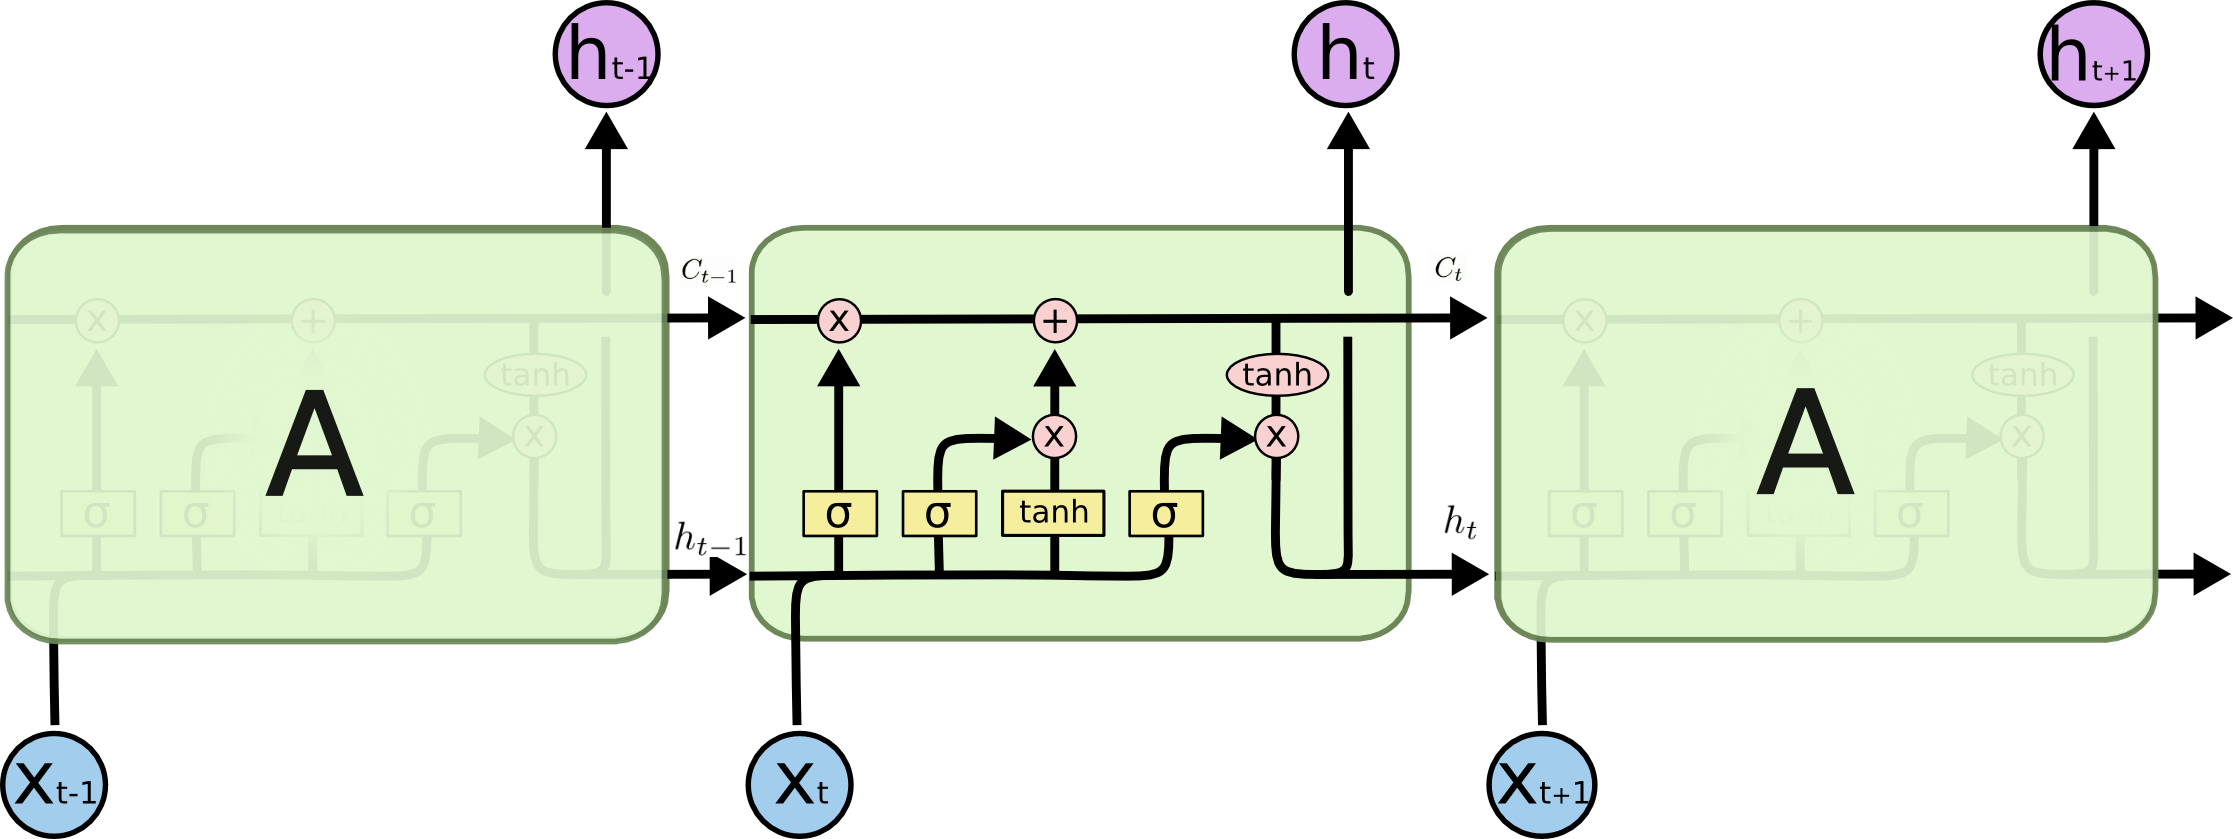
\includegraphics[width=0.7\textwidth]{LSTM3-chain.png}
	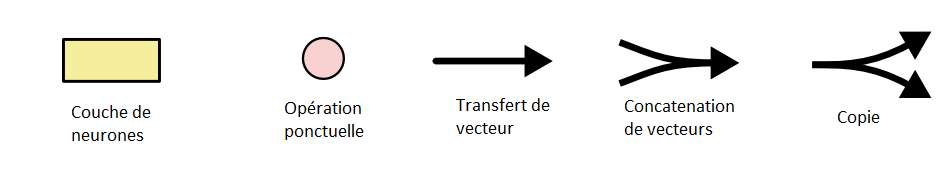
\includegraphics[width=0.7\textwidth]{LSTM2-notation.png}
	
\textit{\scriptsize{\textbf{Source}: \url{https://colah.github.io/posts/2015-08-Understanding-LSTMs/}}}
	\caption{Structure interne d'un LSTM dans une couche de réseau LSTM.}\label{fig:structuration:couchedelstm}
\end{figure}


Les entrées et sorties d'un LSTM sont des vecteurs de nombres réels. L'entrée $X_i$ est la représentation vectorielle indépendante de la séquence entrée de l'observation en position $i$, par exemple celle du mot $t_i$ du texte $T=t_{1:n}$. La sortie $h_i$ représente le contexte de l'observation en position $i$ dans la séquence entrée. On peut ainsi chaîner des LSTM pour modéliser les textes entrées et y appliquer un CRF pour l'étiquetage. C'est le principe du BiLSTM-CRF de \citet{lample2016nnner} une des architectures les plus efficaces pour la l'étiquetage d'entités nommées. En effet, le BiLSTM comprend deux couches enchaînant des LSTM (\figureref{fig:structuration:bi-lstm}). Une couche permet d'apprendre le contexte "gauche" des mots, les états étant propager dans le sens du début vers la fin du texte. L'autre couche apprend le contexte droit en propageant les informations dans le sens inverse. Les mots sont représentées en entrée sous forme vectorielle. Sur la \figureref{fig:structuration:bi-lstm} par exemple, il s'agit de la concaténation du plongement lexical des mot par la méthode Glove \citep{pennington2014glove} et de la représentation contextuelle des caractères dans le mot (\textit{Chars representation}).  

\begin{figure}[!htb]
	\centering 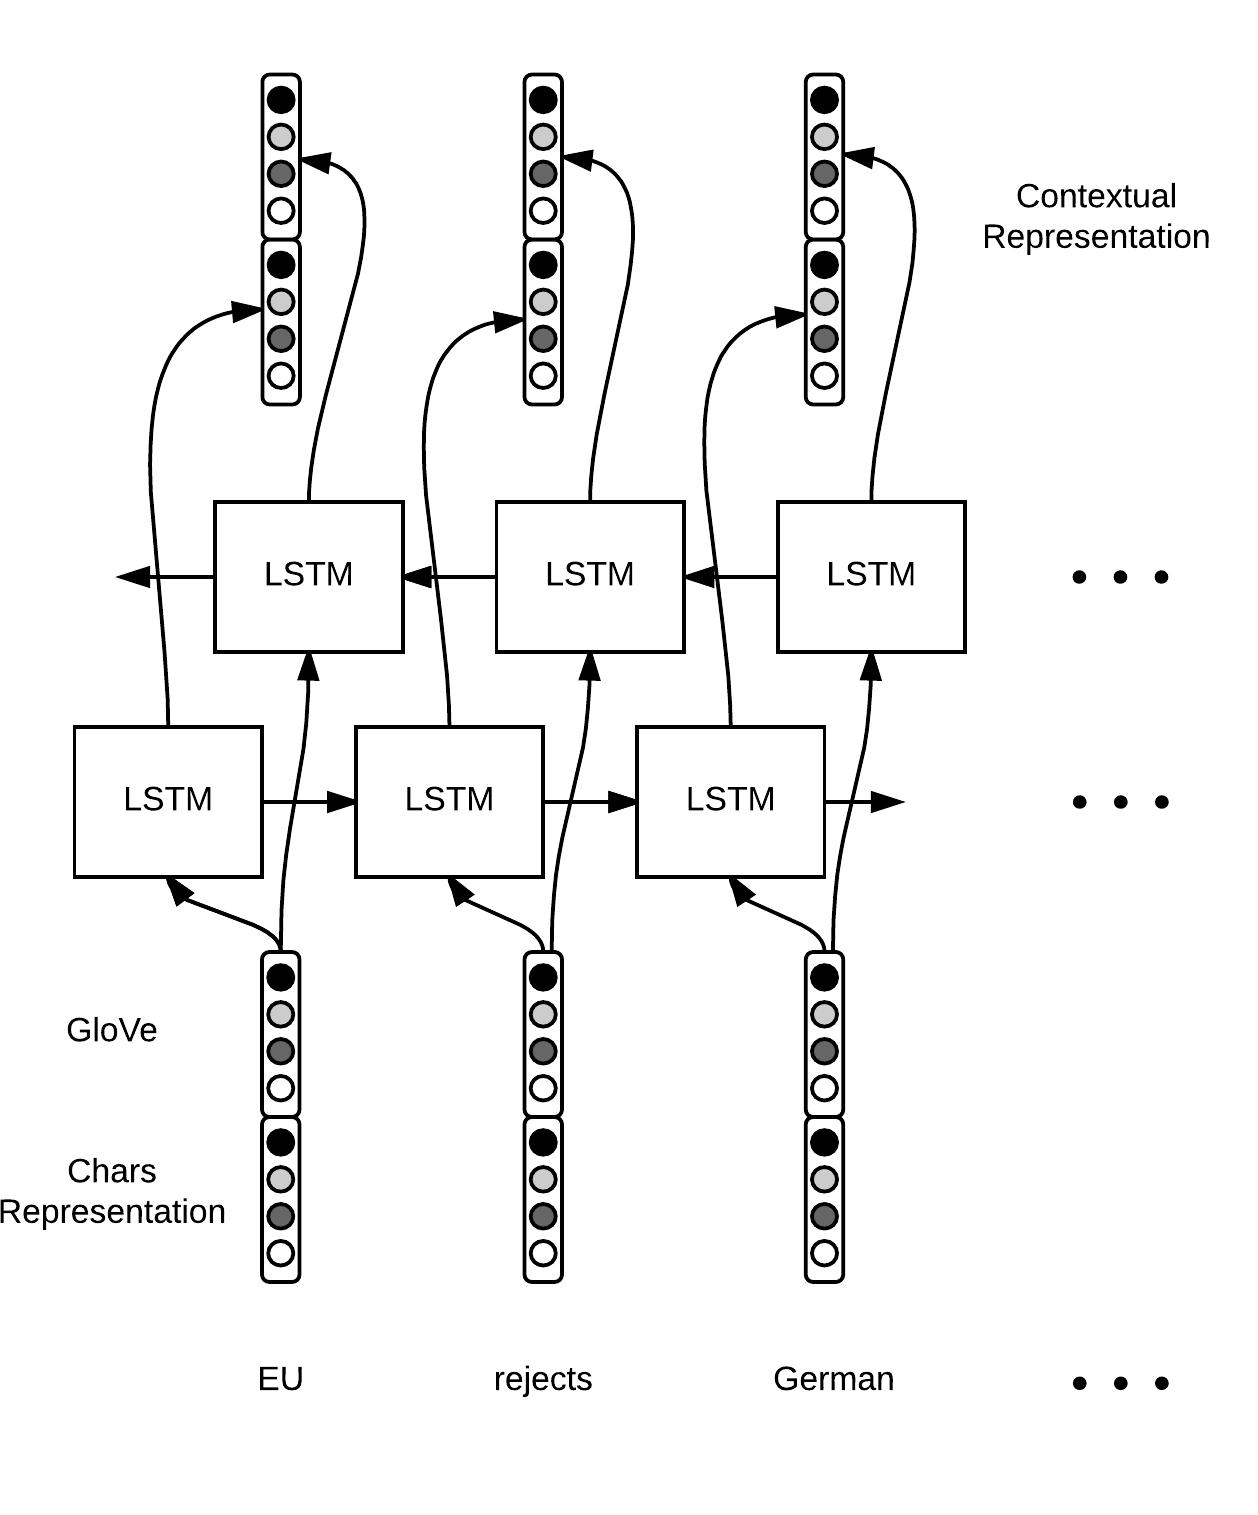
\includegraphics[width=0.7\textwidth]{bi-lstm.png}
		
	\textit{\scriptsize{\textbf{Source}: \url{https://guillaumegenthial.github.io/sequence-tagging-with-tensorflow.html}}}
	\caption{Apprentissage de la représentation contextuelle avec une double couche de réseaux LSTM (BiLSTM).}\label{fig:structuration:bi-lstm}
\end{figure}


\subsection{Représentation des segments atomiques}
%\textcolor{red}{Pourquoi? Quoi ? et Comment?}

La représentation des segments à labelliser occupe une place importante pour l'obtention de bons résultats avec les modèles décrits précédemment. Elle consiste généralement à décrire la forme et le contexte de chaque segment en lui assignant des attributs \citep{nadeau2007nersurvey,sharnagat2014nersurvey}. Ils peuvent être booléens (\og le mot est il en majuscule? \fg{}), numériques (nombre de caractères du mot), nominaux (par ex. le rôle grammatical d'un mot), ou définis par des expressions régulières (par ex. pour les numéros R.G. on peut avoir \verb|dd/ddddd| où \verb|d| désigne un chiffre). Ces descripteurs mettent  en évidence des régularités relatives à l'occurrence des entités. Par exemple, préciser qu'un mot débute par une lettre majuscule permet d'indiquer les noms propres. La définition de tels descripteurs consiste ainsi à fournir au modèle des indices l'aidant à mieux distinguer les différents types d'entités. 

Etant donné que les descripteurs dépendent généralement de l'intuition du concepteur du système d'étiquetage, il est difficile mais nécessaire d'identifier des descripteurs appropriés. Après avoir défini des candidats, il n'est pas sûr qu'en les combinant tous ensemble, on obtienne les meilleures performances. Une sélection de caractéristiques peut alors s'avérer nécessaire. Cette sélection peut améliorer les performances d'étiquetage, et accélérer l'extraction des descripteurs, l'entraînement du modèle, ainsi que son application à de nouveaux textes \citep{kitoogo2007featureSelectNER}. Elle peut aussi fournir une meilleure compréhension du comportement des modèles entraînés \citep{klinger2009FeaturefilterCRF}. Deux principales approches se distinguent. D'une part, les méthodes \og filtrantes \fg{} (\textit{filters}), comme l'information mutuelle, comparent individuellement les descripteurs à l'aide de scores qui ne sont pas nécessairement basés sur la performance. D'autre part, les méthodes \og enveloppantes \fg{} (\textit{wrappers}) comparent des sous-ensembles de descripteurs sur la base des performances d'évaluation qu'elles permettent d'obtenir (par exemple la $F_1$-mesure obtenue sur un ensemble d'exemples). Même si les méthodes filtrantes sont plus rapides, elles sont en général moins performantes car elles ne permettent pas d'éviter les redondances, et ne prennent pas en compte l'effet de la combinaison de caractéristiques.
%. Au départ proposés et utilisés en classification multi-dimensionnelle, les algorithmes de sélections de caractéristiques ont été appliqués avec succès pour l'extraction d'entités. \citet{klinger2009FeaturefilterCRF} ont 

La définition manuelle des caractéristiques suivie de la sélection est souvent qualifiée de méthode forcée car elle dépend fortement de la capacité du concepteur du système à identifier les descripteurs appropriés. 

%2015 https://arxiv.org/pdf/1508.01991.pdf
%https://github.com/UKPLab/emnlp2017-bilstm-cnn-crf
%dnn crf : https://pdfs.semanticscholar.org/c322/7702dd212965157a615332f3dd78b0f11b5e.pdf
%https://towardsdatascience.com/conditional-random-field-tutorial-in-pytorch-ca0d04499463

\subsection{Schéma d'étiquetage}
Nous traitons d'entités dont les occurrences comprennent un ou plusieurs éléments atomiques. Pour améliorer les résultats d'un modèle d'étiquetage, certaines parties des entités peuvent être mises en évidence à travers une représentation appropriée de segments. La \figureref{p4_sample-tagmod} illustre l'utilisation la différence entre des schémas appelés IO, BIO, IEO et BIEO, sur un extrait de décision de justice pour l'annotation du nom d'un juge et de sa fonction.
\begin{figure}[!ht]
	\scriptsize
	\begin{tabular}{l|ccccccccc}
		& \textit{composée} & \textit{de} & \textit{Madame} & \textit{Martine} & \textit{JEAN} & , & \textit{Président} & \textit{de} & \textit{chambre} \\ 
		IO & O & O & I-JUGE & I-JUGE & I-JUGE & O & I-FONCTION & I-FONCTION & I-FONCTION \\
		BIO & O & O & B-JUGE & I-JUGE & I-JUGE & O & B-FONCTION & I-FONCTION & I-FONCTION \\
		IEO & O & O & I-JUGE & I-JUGE & E-JUGE & O & I-FONCTION & I-FONCTION & E-FONCTION\\
		BIEO & O & O & B-JUGE & I-JUGE & E-JUGE & O & B-FONCTION & I-FONCTION & E-FONCTION \\
	\end{tabular}
	\caption{Illustration des schémas d'étiquetage IO, BIO, IEO, BIEO}\label{p4_sample-tagmod}
\end{figure}

Nous comparons dans cette étude quelques schémas d'étiquetage dont certains sont décrits par \citet{konkol2015tagModel}. Le principe de ces schémas est d'étiqueter différemment des segments atomiques en fonction de leur position dans l'entité. Pour cela, le label associé à l'entité est préfixé par l'une des lettres suivantes :

\begin{itemize}
	\item B:  début (\textit{beginning});
	\item I: intérieur (\textit{inside});
	\item E (ou L, ou M) : fin (\textit{end} ou \textit{last} ou \textit{middle});
	\item S (ou U, ou W): singleton ou entité à segment unique (\textit{single} ou \textit{unit} ou \textit{whole});
	\item O: hors de toute entité (\textit{outside}).
\end{itemize}

Le schéma IO utilisé par défaut ne met l'accent sur aucune partie et affecte le même label à tous les segments d'une même entité. D'autres schémas distinguent soit le premier élément (BIO), soit le dernier (IEO), soit les deux (BIEO). Les schémas IEO et BIO ont des variantes IEO1, BIO1, IOE2, et BIO2. Les modèles IOE2, et BIO2 utilisent resp. les préfixes E- et B- pour étiqueter les entités à mot unique, contrairement à IEO1 et BIO1 qui utilisent plutôt le préfixe I- dans ce cas. Le modèle BIEO est souvent étendu sous la forme BIESO (ou BILOU) dans le cas où l'on souhaite distinguer les entités à un seul segment (par ex. ville ou numéro R.G.). Il est possible d'aller plus loin en mettant l'accent sur les mots avant  (O-JUGE) et après (JUGE-O) l'entité (JUGE par exemple) et en indiquant le début (BOS-O, \textit{begininning of sentence}) et la fin (O-EOS, \textit{end of sentence}) du texte ou de la phrase. Le format ainsi obtenu est appelé BMEWO+ \citep{baldwin2009bmewo}.

Un autre intérêt des schémas plus complexes que IO est de pouvoir distinguer des entités du même type qui se suivent sans être explicitement séparées (par exemple, des appelants mentionnés sur des lignes consécutives). Cet aspect est notamment important dans les décisions de justice par exemple lorsque des noms de parties sont listés dans la section ENTETE en n'étant séparés que d'un simple retour à la ligne.

\section{Architecture proposée}
\label{sec:structuration:proposition}
\begin{figure}[!htb]
%\sidecaption
\begin{center}
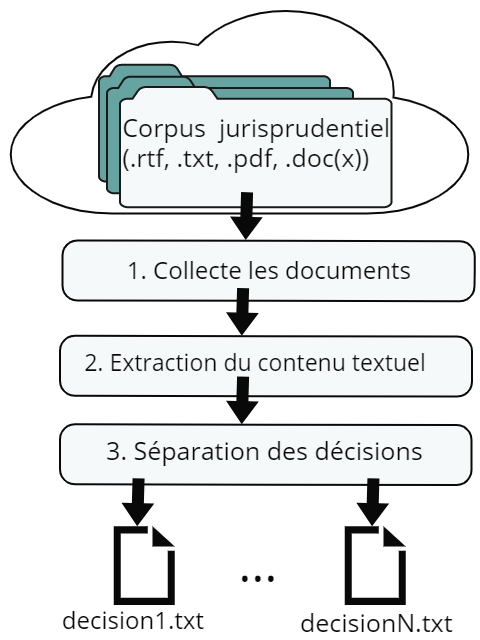
\includegraphics [width=0.45\textwidth]{structuration-preprocess.png}
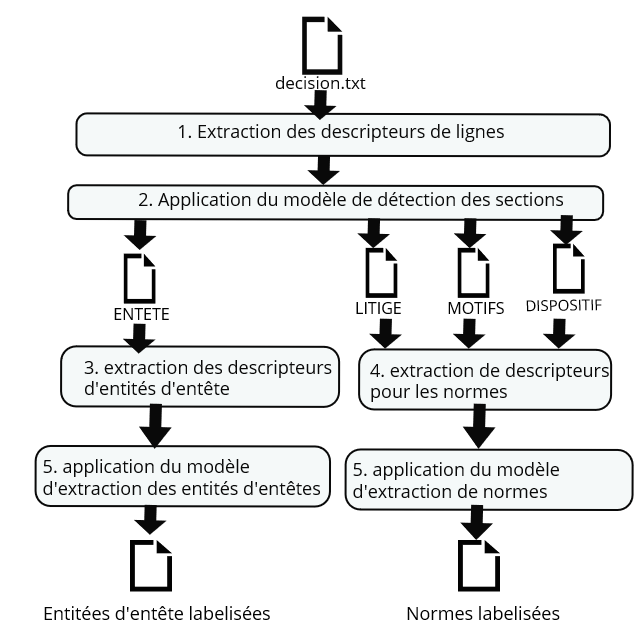
\includegraphics [width=0.45\textwidth]{structuration-pipeline-application.png}
\end{center}

{\footnotesize Après la collecte et le pré-traitement des documents, l'étiqueteur de ligne est d'abord appliqué pour détecter les sections, puis les étiqueteurs d'entités peuvent être appliqués simultanément dans les sections.}
\caption{Application des modèles entraînés pour l'étiquetage de sections et entités.}\label{fig:structuration:archAppli}
\end{figure}
Nous proposons de travailler uniquement avec le contenu textuel des documents. Ce contenu est extrait des documents téléchargés en éliminant les éléments inutiles, principalement des espaces vides. Ces éléments sont typiques des documents formatés (\verb|.rtf, .doc(x), .pdf|). Ils ne fournissent pas une indication standard sur le début des sections. Le choix de ne pas exploiter le formatage des documents permet d'avoir à gérer un nombre plus faible de diversités entre les textes tout en appliquant le même processus de traitement à tout document indépendamment de son format d'origine. Une simple architecture d'étiquetage de sections et d'entités juridiques a été conçue avec cette uniformisation des documents comme point d'entrée (\figureref{fig:structuration:archAppli}). Ainsi, les documents sont collectés puis pré-traités suivant leur format d'origine (extraction du texte et séparation des décisions apparaissant dans le même document).  Ensuite, après le sectionnement des décisions, les entités sont identifiées dans les différentes sections. Par ailleurs, comme segment atomique à étiqueter nous avons choisi les lignes pour la détection des sections, et les mots pour les entités. 

\begin{figure}[!ht]
%\sidecaption
\centering
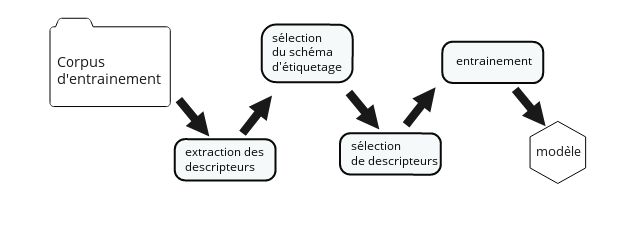
\includegraphics [width=\textwidth]{structuration-training.png}
\caption{Entrainement des modèles.}\label{fig:structuration:training}
\end{figure}


Les modèles HMM et CRF étant tous les deux supervisés, ils doivent être entraînés sur des exemples manuellement annotés pour estimer leurs paramètres. Nous proposons de sélectionner le schéma d'étiquetage et les sous-ensembles minimaux de caractéristiques manuellement définies, avant d'entraîner les modèles HMM et CRF (\figureref{fig:structuration:training}). 

\subsection{Définition manuelle de descripteurs candidats}

\subsubsection{Descripteurs pour la détection des sections}

\begin{table}[!htb]
	\centering
	\begin{tabular}{|l|l|}
		\hline
		\multicolumn{1}{|c}{Type} & \multicolumn{1}{|c|}{Descripteur} \\ \hline
		Forme & \tabitem la ligne entière (\verb|token|)  \\  
		& \tabitem ses premiers mots (\verb|t0, t1, t2|) \\
		& \tabitem sa longueur absolue (\verb|absLength|) \\ 
		& \tabitem sa longueur relative (\verb|relLength|) \\ \hline
		Contexte & \tabitem le numéro de ligne (\verb|absNum|) \\
		& \tabitem partie du document contenant la ligne (\verb|relNum|) \\
		& \tabitem premiers mots de la ligne précédente (\verb|p0, p1|) \\ 
		& \tabitem premiers mots de la ligne suivante (\verb|n0, n1|) \\
		& \tabitem longueur absolue de ligne précédente (\verb|nLength|) \\  
		& \tabitem longueur relative de ligne précédente (\verb|nRelLength|) \\
		& \tabitem longueur absolue de ligne suivante (\verb|nLength|) \\  
		& \tabitem longueur relative de ligne suivante (\verb|nRelLength|) \\ \hline
	\end{tabular}
	\caption{Descripteurs candidats de lignes pour les sections.} \label{tab:structuration:descripteursligne}
\end{table}

Nous considérons donc la ligne comme élément à étiqueter lors du sectionnement. Nous n'avons pas travaillé au niveau des mots afin d'éviter que des mots de la même ligne ne soient classés dans des sections différentes. L'étiquetage des phrases a aussi été évité car en découpant les documents en phrases telles qu'elles sont entendues en français, on a parfois des segments qui s'étendent d'une section à une autre (absence de ponctuation). De plus, l'entête à davantage l'apparence d'un formulaire.

Plusieurs critères peuvent être utilisés pour différencier les sections, à savoir: la longueur des lignes (plus longues dans le corps, plus courtes dans l'entête), les premiers termes de certaines lignes (typiques de chaque section) et le nombre total de lignes. Un HMM ne supporte qu'un descripteur représentant l'élément à étiqueter. D'autres descripteurs peuvent être la position de l'élément à étiqueter (numéro de ligne) ou le début de la ligne. Le descripteur capturant la longueur de ligne peut être absolu (nombre exact de mots dans la ligne), ou relatif (une catégorie de la longueur). Sur la base des quantiles de la distribution des longueurs de lignes sur un ensemble de décisions, nous avons défini trois catégories:
\verb|LQ1| ($longueur \leq$ 5), \verb|LQ2| (5 < $longueur \leq$ 12) et \verb|LQ2| (12 < $longueur \leq$ 14). Nous avons également catégorisé les parties du document afin de capturer une position relative de ligne.
En effet, le document est considéré comme divisé en $N$ parties (10 dans nos expériences). La position relative d'une ligne est donc le numéro de la partie contenant la ligne. Les descripteurs représentant les lignes sont résumés dans le \tableref{tab:structuration:descripteursligne}.

\subsubsection{Descripteurs pour la détection d'entités}

La détection d'entités consiste, dans notre cas, à entraîner un modèle CRF ou HMM pour étiqueter les différents segments de texte (mot, ponctuation, numéro, identifiant) suivant qu'ils appartiennent ou non à la mention d'une entité. Les deux modèles nécessitent des caractéristiques, dont certaines peuvent être définies sur la base de régularités directement observables dans les textes. Sur la base des observations de décision, nous avons défini la morphologie des mots en décrivant la forme des caractères du mots. Le lemme est aussi utilisé car il homogénéise les variantes du mot correspondant. Pour identifier les normes,  nous définissons une liste de mots utilisés pour citer les règles juridiques (\textit{article, code, loi, contrat, décret, convention, civil, pénal}, etc.). Cette liste permet d'indiquer si le mot est décrit est un mot-clé de norme. Le contexte des mots est défini en plus de la forme en décrivant les mots voisins. Par ailleurs, la position des mots par rapport à certains termes-clés semble indiquer la nature potentielle de ces mots. Par exemple, les appelants sont généralement listés avant le mot \textit{appelants} et après le mot \textit{intimés}.
Il est également possible d'obtenir des descripteurs à partir du résultat d'autres tâches d'analyse de texte dont les rôles grammaticaux (\textit{Part-of-Speech}) comme \citet{chang2005applyingNER} et les modèles thématiques (\textit{topic model}) comme \citet{polifroni2011usingLDA} et \citet{nallapati2010blinddomaintransferner}. Le \tableref{tab:structuration:descripteursmots} résume l'ensemble des descripteurs caractéristiques définis pour la détection des entités.
%Les rôles grammaticaux peuvent être intéressants par exemple pour identifier les noms de personnes et de villes dont les mots dont le rôle est généralement ??. Le thème d'un mot 

%\textbf{Rôles grammaticaux} : certaines entités ont tendance à contenir des rôles grammaticaux particuliers. Par exemple, les noms d'individus sont composés de noms propres . Nous avons extrait le rôle grammatical du mot courant (\verb|POS|) ainsi que celui de ses voisins (\texttt{POSW-2, POSW-1, POSW1, POSW2}).
%
%\textbf{Modèles thématiques}: comme \citet{polifroni2011usingLDA} et \citet{nallapati2010blinddomaintransferner}, nous utilisons des associations mot-thème pour décrire les mots. Il s'agit de modéliser un ensemble de $N$ thèmes et d'utiliser leurs identifiants comme descripteurs. Il serait peut-être intéressant d'utiliser la probabilité déduite du modèle thématique, mais l'inférence sous-jacente au modèle LDA \citep{blei2003lda} n'est pas déterministe (la distribution de probabilité change pour le même mot entre différentes inférences).
%Néanmoins, l'ordre des sujets ne changeant pas de manière significative, nous avons utilisé l'identifiant du thème le plus pertinent pour le mot (\verb|topic0|) ainsi que ceux de ses voisins (\verb|w-2topic0|, \verb|w-1topic0|, \verb|w1topic0|, \verb|w2topic0|).

\begin{table}[!htb]
	%\centering 
	\small
	\begin{tabular}{|l|p{0.78\textwidth}|}
		\hline
		\multicolumn{1}{|c|}{Type} & \multicolumn{1}{c|}{Descripteur} \\ \hline
Forme & \tabitem le mot (\verb|token|)  \\ 
	& \tabitem son lemme (\verb|lemma_W0|) \\
	& \tabitem \og commence-t-il par une lettre majuscule ? \fg{} (\verb|startsWithCAP|) \\
	&\tabitem\og est-il entièrement en majuscule ? \fg{} (\verb|isAllCAP|)\\
	&\tabitem\og est-ce une initiale solitaire tel que "B."? \fg{} (\verb|isLONELYINITIAL|)\\
	& \tabitem \og contient-il un caractère de ponctuation ? \fg{} (\verb|PUN-IN|) \\
	& \tabitem \og n'est-ce qu'une ponctuation ? \fg{} (\verb|isALLPUN|) \\
	& \tabitem \og contient-il un caractère numérique ? \fg{} (\verb|DIGIT-IN|) \\
	& \tabitem \og ne contient-il que 
des chiffres ? \fg{} (\verb|isALLDIGIT|) \\ 
	& \tabitem \og S'agit-il d'un mot-clé de règles juridiques ? \fg{} (\verb|isKEYWORD|) \\ \hline
Syntaxe & \tabitem rôle grammatical du mot (\verb|POS|) \\ \hline
Sémantique & \tabitem thème du mot (\verb|topic0|) \\  \hline
Contexte & \tabitem les mots précédents (\verb|w-1, w-2|) \\
		& \tabitem les lemmes des mots précédents  (\verb|lemmaW-1, lemmaW-2|) \\
	& \tabitem les mots suivants (\verb|w1, w2|) \\
	& \tabitem les lemmes des mots suivants  (\verb|lemmaW1, lemmaW2|) \\
	& \tabitem numéro de ligne (\verb|lineNum|) \\ 
	& \tabitem position de l'élément dans la ligne (\verb|numInLine|) \\
	& \tabitem \og le document contient-il le mot \textit{intervenant} ? \fg{} \\
	& (\verb|intervenantInText|) \\
	& \tabitem \og le mot apparaît-il après \textit{APPELANT}, \textit{ENTRE}, et \textit{DEMANDEUR} ? \fg{} (\verb|isAfterAPPELANT|) \\
	& \tabitem \og le mot apparaît-il après \textit{INTIME}, \textit{ET}, et \textit{DEFENDEUR} \fg{} (\verb|isAfterINTIME|)\\
	& \tabitem \og le mot apparaît-il après  \textit{INTERVENANT} ? \fg{} \\ 
	& (\verb|isAfterINTERVENANT|) \\
	& \tabitem numéro de la ligne précédente contenant le mot (\verb|lastSeenAt|)\\
	& \tabitem nombre d'occurrences du mot (\verb|nbTimesPrevSeen|)\\
	& \tabitem rôles grammaticaux des mots voisins (\texttt{POSW-2, POSW-1,} \\ 
	& \texttt{POSW1, POSW2}) \\ 
	& \tabitem thèmes des mots voisins (\verb|w-2topic0|, \verb|w-1topic0|, \verb|w1topic0|, \verb|w2topic0|) \\ 
	 \hline
	\end{tabular}	
	\caption{Descripteurs candidats de mots pour les mentions d'entités.} \label{tab:structuration:descripteursmots}
\end{table}

\subsection{Sélection des descripteurs}
\subsubsection{Sélection  pour le modèle CRF}
 Nous avons étudié deux approches enveloppantes qui semblent toujours converger et qui ne nécessitent pas de définir manuellement la taille du sous-ensemble cible. %Il s'agit de la recherche bidirectionnelle et de la  sélection séquentielle à flottement avant. 

\begin{algorithm}[ht] \small
	\KwData{Données annotées, $X$ liste de tous les descripteurs candidats}
	\KwResult{Meilleur sous-ensemble de descripteurs}
	Démarrer la SFS avec $Y_{\mathcal{F}_0}= \emptyset $\; 
	Démarrer la SBS avec $Y_{\mathcal{B}_0}=X$\; $k=0$\;
	\While{$Y_{\mathcal{F}_k} \neq Y_{\mathcal{B}_k}$}{
		$x^+=\argmax_{\substack{x \in Y_{\mathcal{B}_k} \setminus Y_{\mathcal{F}_k}}} F_1(Y_{\mathcal{F}_k} + x)$; 
		$Y_{\mathcal{F}_{k+1}} = Y_{\mathcal{F}_k} + x^+$ //SFS\;
		$x^-=\argmax_{\substack{x \in Y_{\mathcal{B}_k} \setminus Y_{\mathcal{F}_{k+1}}}} F_1(Y_{\mathcal{F}_k} - x)$;
		$Y_{\mathcal{B}_{k+1}} = Y_{\mathcal{B}_k} - x^-$ //SBS\; 
		$k = k+1$;
	}
	\Return $Y_{\mathcal{F}_k}$\;
	\caption{Recherche bidirectionnelle BDS} \label{algo:structuration:bds}
\end{algorithm}
La première méthode, qui est la recherche bidirectionnelle (BDS) de \citet{liu2012featureSelection}, combine la sélection séquentielle en avant (SFS) et la sélection séquentielle en arrière (SBS) en parallèle (Algorithme \ref{algo:structuration:bds}). 
La SFS recherche un sous-ensemble optimal, en commençant par un ensemble vide et en ajoutant le descripteur qui améliore le mieux l'efficacité du sous-ensemble sélectionné. Le critère d'efficacité dans notre cas est défini par la $F_1$-mesure (Eq. \ref{eq:structuration:f1mesure}). Contrairement à la SFS, la SBS commence par l'ensemble des candidats et supprime successivement les plus mauvais descripteurs. Une caractéristique ne peut être ajoutée dans $Y_{F_{k+1}}$ que si elle est présente dans $Y_{B_{k}}$.



\begin{algorithm}[ht] %\small
	\KwData{Données annotées, $X$ liste de tous les descripteurs candidats}
	\KwResult{Meilleur sous-ensemble de descripteurs}
	$Y_0= \emptyset $\; 
	$k=0$\;
	\Repeat{$X = \emptyset$ ou $X = Y_{k}$}{
		$x^+=\argmax_{x \notin Y_k} F_1(Y_k + x)$; \label{p4_forward_sffs}
		$Y_k = Y_k + x^+$\; 
		$x^-=\argmax_{x \in Y_k} F_1(Y_k - x)$\; \label{p4_back_sffs}
		\eIf{$F_1(Y_k - x^-) > F_1(Y_k)$}{
			$Y_{k+1} = Y_k - x^-$\; 
			$X = X - x^-$\;
			$k = k+1$\;
			Rentrer à \ref{p4_back_sffs}\;
		}{
			Rentrer à  \ref{p4_forward_sffs}\;
		}
	}
	\Return $Y_k$\;
	\caption{Sélection séquentielle avant à flottement}\label{algo:structuration:sffs}
\end{algorithm}

La seconde méthode, qui est l'algorithme de sélection séquentielle avant à flottement SFFS  de \citet{pudil1994floatingFeatSelection}, étend la SFS en surmontant son incapacité à réévaluer l'utilité d'un descripteur après son rejet (Algorithme \ref{algo:structuration:sffs}). En effet, le SFFS effectue des tests en arrière à chaque itération.

\subsubsection{Sélection pour le modèle HMM} Pour sélectionner les meilleurs descripteurs pour les modèles HMM, nous avons testé individuellement les différents candidats. La caractéristique donnant le meilleur résultat sur l'ensemble de données annotées est sélectionnée.

\section{Expérimentations et discussions}

L'objectif de cette section est de discuter des différents aspects liés à la performance des modèles CRF et HMM. Il est question de discuter l'effet des descripteurs candidats définis, de comparer des algorithmes de sélection de caractéristiques et des schémas d'étiquetage. Nous discutons par la suite l'origine des erreurs (confusion, nombre d'exemples d'entraînement), et comparons les descripteurs définis manuellement par rapport à l'utilisation de réseaux de neurones.

\label{sec:structuration:experimentations}
\subsection{Conditions d'expérimentations}
\subsubsection{Annotation des données de référence}
Pour évaluer les méthodes de TAL, \citet{xiao2010corpuscreation} suggère de choisir un jeu d'exemples suffisant en assurant au mieux l'équilibre dans la variété des données et la représentativité du langage. Nous avons essayé de suivre cette recommandation  en sélectionnant aléatoirement des décisions à annoter. Au total, 503 documents ont été rassemblés et annotés manuellement à l'aide de la plateforme GATE Developer\footnote{https://gate.ac.uk/family/developer.html}. Cet outil permet de marquer les passages à annoter en les surlignant à l'aide du pointeur de la souris; ce qui allège  l'annotation manuelle. Des balises XML sont rajoutées autour des passages sélectionnés, en arrière plan dans le document.

Chaque document annoté comprend en moyenne 260 lignes et 3900 mots environ. Les deux dernières colonnes du \tableref{tab:structuration:relevantinfo} présentent la distribution des entités labellisées dans le jeu de données. En se basant sur un sous-ensemble de 13 documents labellisés par 2 annotateurs différents, nous avons calculé des taux d'accord inter-annotateur en utilisant la statistique Kappa de \citet{cohen1960kappa}. Ces mesures d'accord inter-annotateur ont été calculées au niveau des caractères parce que certains mots peuvent être coupés par des annotations incorrectes (par ex. \textit{<juridiction> cour d'appe </juridiction> \underline{l}} contre \textit{<juridiction> cour d'appe\underline{l} </juridiction>}), ou bien les annotateurs pourraient ne pas être d'accord si une apostrophe devrait être incluse ou pas dans l'annotation (par ex. \textit{ \underline{l'}<norme>article 700} contre \textit{ <norme >\underline{l'}article 700}). Les taux de Kappa de 0,705 et 0,974 ont été obtenus pour l'annotation des entités et des sections respectivement. D'après la catégorisation de \citet{viera2005kappa}, le niveau d'accord observé est \textit{substantiel} pour les entités (0,61 -- 0,80) et \textit{presque parfait} pour les sections (0,81 -- 0,99).

\subsubsection{Mesures d'évaluation}
Nous avons utilisé la précision, le rappel et la $F_1$-mesure comme mesures d'évaluation car elles sont généralement utilisées comme références en extraction d'information. % Nous présentons aussi des performances au niveau micro c'est-à-dire en général sans distinction des classes. 
La $F_1$-mesure se calcule à l'aide de la formule suivante:  
\begin{equation}\label{eq:structuration:f1mesure}
F_1 = 2 \times \frac{Precision \times Rappel} {Precision + Rappel}.
\end{equation}
%La précision et le rappel quant à eux se calculent suivant les formules
% \begin{equation}\label{NER-precision}
% Precision = \frac{TP}{}
% \end{equation}

L'évaluation peut être faite au niveau des segments atomiques ou  des entités selon que l'on soit plus intéressé respectivement par l'étiquetage  du maximum de segments atomiques ou par la labellisation complète d'un maximum d'entités.

\noindent \underline{\textbf{Evaluation au niveau atomique (\textit{token-level)}}}: cette évaluation mesure la capacité d'un modèle à labelliser les segments atomiques des entités. Les valeurs de précision et rappel sont calculées sur les données de test pour chaque label $l$ comme suit:

\[Precision_l = \frac{\text{nombre de segments correctement labellisés par le modèle avec } l} {\text{nombre de segments labellisés par le modèle avec } l}\]
\[Rappel_l = \frac{\text{nombre de segments correctement labellisés par le modèle avec } l} {\text{nombre de segments manuellement labellisés avec } l}\]

\vspace{0.3cm}

\noindent \underline{\textbf{Evaluation au niveau entité (\textit{entity-level})}}: cette évaluation mesure le taux d'entités parfaitement identifiées c'est-à-dire seulement celles dont les segments atomiques ont été tous correctement labellisés. Les valeurs de précision et rappel sont calculées sur les données de test pour chaque classe d'entité $e$ comme suit :
\[Precision_e = \frac{\text{nombre d'entités de type } e \text{ parfaitement détectées par le modèle}} {\text{nombre d'entités détectées et classifiées } e\text{ par le modèle}}\]
\[Rappel_e = \frac{\text{nombre d'entités de type } e \text{ parfaitement détectées par le modèle}} {\text{nombre d'entitées manuellement classifiées } e}\]

\vspace{0.3cm}

\noindent \underline{\textbf{Evaluation globale (\textit{overall-level})}} : l'évaluation globale donne les performances générales d'un modèle sans distinction des classes ou labels. Elle est réalisée aux deux niveaux décrits précédemment mais indépendamment du label d'élément ou du type d'entité. La précision et le rappel sont calculées au niveau des entités comme suit :
\[Precision = \frac{\text{nombre d'entités correctement labellisées par le modèle}} {\text{nombre d'entités labellisées par le modèle}}\]
\[Rappel = \frac{\text{nombre d'entités correctement labellisées par le modèle}} {\text{nombre d'entités  manuellement labellisées}}.\]
Ces métriques sont calculées de la même façon au niveau atomique.

\subsubsection{Outils logiciels}
Nous avons utilisé les modèles HMM et CRF tels qu'implémentés dans la librairie Mallet \citep{McCallum2012Mallet}. Les modèles étudiés ont été entraînés par la méthode d'espérance maximale pour ceux basés sur le HMM, et par la méthode L-BFGS pour ceux basés sur le CRF. Le découpage des textes en mots (\textit{tokenisation}), la lemmatisation, et l'annotation des rôles grammaticaux (\textit{Part-of-Speech tagging}) ont été effectués à l'aide de la fonctionnalité d'annotation de textes français de TreeTagger \footnote{\url{http://www.cis.uni-muenchen.de/~schmid/tools/TreeTagger}}  \citep{schmid1994treetagger}. L'implémentation dans Mallet du LDA \citep{blei2003lda} a permis d'inférer 100 thèmes à partir d'un corpus lemmatisé d'environ 6k documents. Le \tableref{p4_topics} 
présente des mots représentatifs trouvés dans les premiers thèmes inférés. L'extraction des autres descripteurs a été implémentée pour cette expérimentation. 


\begin{table}[!ht]
\small
\begin{center}
\begin{tabular}{c|p{0.8\textwidth}}
Id thème & Mots représentatifs  \\ \hline
0	& 	préjudice  dommage  somme  subir  réparation  titre  faute  payer  intérêt  responsabilité  \\ \hline
1	& société  salarié  groupe  mirabeau  pouvoir  demande  article  licenciement  cour  titre    \\ \hline
2	& harcèlement  travail  salarié  moral  employeur  fait  attestation  faire  santé  agissements  \\ \hline
3	& vente  acte  prix  vendeur  acquéreur  notaire  condition  clause  vendre  immeuble  \\ \hline
4	& 		travail  poste  reclassement  employeur  médecin  licenciement  salarié  inaptitude  visite  \\ \hline
5	& 	monsieur  nîmes  avocat  appel  barreau  arrêt  madame  disposition  prononcer  président  \\ \hline
6	& 	mademoiselle  madame  non  mesure  décision  tutelle  surendettement  comparant   \\ \hline
7	& transport  marchandise  jeune  sed  éducateur  bateau  navire  transporteur  responsabilité  \\ \hline
8	&congé  salarié  conversion  emploi  plan  convention  employeur  sauvegarde  reclassement  \\ \hline
9	&marque  site  contrefaçon  sous  droit  auteur  joseph  produit  propriété  photographie  \\ \hline
10	&pierre  patrick  bordeaux  bruno  catherine  civil  article  corinne  cour  avocat\\ \hline
\end{tabular}
\end{center}
\caption{Mots représentatifs des 10 premiers thèmes sur les 100 inférés}\label{p4_topics}
\end{table}

Les valeurs de précision, rappel, et $F_1$-mesure ont été calculées à l'aide du script d'évaluation de la campagne CoNLL-2002 \footnote{\url{http://www.cnts.ua.ac.be/conll2002/ner/bin/conlleval.txt}}. Elles sont indiquées en pourcentage dans les tableaux de résultats d'évaluation des sections suivantes.

\subsection{Sélection du schéma d'étiquetage}
Dans le but d'évaluer comment la représentation de segments affecte les performances, nous avons implémenté quatre représentations (IO, IEO2, BIO2, BIEO).  Nous avons réalisé un simple découpage des données en deux ensembles: $25 \%$ pour l'entraînement et $75 \%$ pour les tests. Les performances reportées dans le \tableref{fig:structuration:select-segm-repr} sont les performances globales sur la base de test. Seul l'élément (mot/ligne) est utilisé comme descripteur. La durée d'entraînement est très longue, particulièrement pour la détection d'entités dans l'entête avec le CRF. Il semble évident que cette durée croisse avec le nombre de labels candidats de la section et la complexité du schéma d'étiquetage. En effet, BIEO exige beaucoup plus de temps, et IO exige le temps d'entraînement le plus bas, et le schéma IOE semble être plus rapide que BIO même s'ils ont le même nombre de labels. Nous remarquons aussi que les représentations complexes n'améliorent pas significativement les résultats par rapport au simple IO qui demande pourtant beaucoup moins de temps.

\begin{table}[ht]
\scriptsize
\begin{center}
\begin{tabular}{p{0.9cm}|c|cccccccc}
\hline \noalign{\smallskip}
Tâche & Modèle & \multicolumn{3}{c}{Niveau atomique$^a$} & \multicolumn{3}{c}{Niveau entité$^a$} & \multirow{2}{*}{Durée$^b$} & Schéma \\
 & & Précision & Rappel & $F_1$ &  Précision & Recall & $F_1$ &  & \\ \hline %\noalign{\smallskip}\svhline\noalign{\smallskip}
\multirow{8}{*}{Sections}  & \multirow{4}{*}{CRF} & 91.75 & 91.75 & 91.75 & 64.49 & 56.55 & 60.26 &  4.685  & IO \\
&  & 88.95 & 88.95 & 88.95 & 48.12 & 38.26 & 42.63  & 11.877 & IEO2 \\
&  & 87.09 & 87.09 & 87.09 & 46.79 & 37.20 & 41.45 & 12.256 & BIO2 \\
 &  & 86.00 & 86.00 & 86.00 & 58.98 & 41.86 & 48.97  & 35.981 & BIEO \\ \cline{2-10}
& \multirow{4}{*}{HMM} & 32.64 & 32.64 & 32.64 & 22.16 & 18.91 & 20.41 & 6.564 & IO \\
&  & 32.92 & 32.92 & 32.92 & 17.73 & 16.09 & 16.87  &   7.827  & IEO2 \\
 &  & 32.39 & 32.39 & 32.39 & 31.93 & 26.65 & 29.05 & 8.391 & BIO2 \\
  &  & 33.06 & 33.06 & 33.06 & 32.47 & 27.53 & 29.80 & 8.7 & BIEO \\ \hline %
\multirow{8}{0.9cm}{Entités d'entête}  & \multirow{4}{*}{CRF} & 86.86 & 78.96 & 82.73 & 80.84 & 65.17 & 72.17  & 70.525 & IO \\%\multirow{8}{=}{Entités d'entête}
 &  & 87.77 & 79.65 & 83.51 & 82.46 & 65.19 & 72.82  & 228.751 & IEO2 \\
 &  & 87.41 & 78.14 & 82.51 & 81.66 & 66.80 & 73.49 & 230.865 & BIO2 \\
 &  & 87.72 & 79.55 & 83.44 & 84.38 & 68.35 & 75.53 &  475.249 & BIEO \\ \cline{2-10}
  & \multirow{4}{*}{HMM} & 79.12 & 67.75 & 73.00 & 61.48 & 35.05 & 44.64 & 6.345 & IO \\
  &  & 78.82 & 68.69 & 73.40 & 66.63 & 40.16 & 50.11& 8.298 & IEO2 \\ 
  &  & 80.68 & 67.48 & 73.49 & 70.37 & 45.32 & 55.14 & 7.908 & BIO2 \\
 &  & 80.05 & 69.01 & 74.12 & 74.73 & 50.77 & 60.46 & 9.973 & BIEO \\ \hline
\multirow{8}{*}{Normes}  & \multirow{4}{*}{CRF} & 95.60 & 92.96 & 94.26 & 88.06 & 83.50 & 85.72 & 28 & IO \\%
&  & 95.40 & 93.18 & 94.27 & 88.75 & 85.65 & 87.17 & 32.136 & IEO2 \\
 &  & 95.20 & 93.30 & 94.24 & 85.65 & 83.13 & 84.37 & 50.769 & BIO2 \\
  &  & 95.46 & 91.57 & 93.47 & 88.83 & 84.71 & 86.72 & 50.566 & BIEO \\ \cline{2-10}
  & \multirow{4}{*}{HMM} & 89.83 & 88.78 & 89.30 & 73.74 & 75.02 & 74.37 &  41.389 & IO \\%  
   &  & 88.20 & 89.23 & 88.71 & 78.01 & 81.27 & 79.61 & 44.086 & IEO2 \\
  &  & 89.25 & 87.83 & 88.53 & 73.89 & 76.63 & 75.24 & 46.634 & BIO2 \\
  &  & 87.39 & 88.10 & 87.74 & 77.76 & 82.35 & 79.99 & 45.52& BIEO \\ 
\noalign{\smallskip}\hline\noalign{\smallskip}
\end{tabular}
\end{center}

$^a$ Résultats sur une simple division du jeu de données en $25\%$ pour l'entraînement et  $75\%$ pour les tests (entraînement limité à 100 itérations maximum)

$^b$ Durée d'entraînement en secondes avant l'arrêt de l'entraînement

\caption{Comparaison des schémas d'étiquetage.}\label{fig:structuration:select-segm-repr}
\end{table}


\subsection{Sélection des descripteurs}
Pour comparer les méthodes BDS et SFFS, nous exploitons le schéma IO. Durant nos expérimentations, la méthode SFFS a exécuté 185 entraînements pour le modèle CRF d'identification des sections. La méthode BDS quant à elle a duré plus de 15h pour 600 itérations d'entraînement-test. Malgré la sauvegarde des scores $F_1$ pour éviter d'exécuter plusieurs fois l'entraînement pour les mêmes sous-ensembles de descripteurs, le processus de sélection est toujours resté très long pour les deux algorithmes. Nous avons testé individuellement chacun des descripteurs candidats pour les modèles HMM. Les résultats sont reportés dans le \tableref{fig:structuration:select-feats}.

\begin{table}[!htb]
\scriptsize
\begin{center}
\begin{tabular}{p{1cm}|c|ccc|ccc|c}
\hline\noalign{\smallskip}
Tâche & Modèle & \multicolumn{3}{c}{niveau atomique$^a$} & \multicolumn{3}{c}{niveau entité$^a$}& Sous-ensemble \\
 & & Précision & Rappel & $F_1$ &  Précision & Rappel & $F_1$ & sélectionné\\
\noalign{\smallskip}\hline\noalign{\smallskip}
\multirow{7}{*}{Sections} 		& \multirow{4}{*}{CRF} & 99.31 & 99.31 & 99.31 & 90.28 & 90.68 & 90.48 & BDS$^{b1}$  \\
  				&  & 99.55 & 99.55 & {99.55} & 85.69 & 85.84 & 85.76 & {SFFS}$^{b2}$ \\
                &  & 99.36 & 99.36 & 99.36 & 88.16 & 88.39 & 88.27 & TOUS$^{b0}$ \\
                &  & 91.75 & 91.75 & 91.75 & 64.49 & 56.55 & 60.26 & token \\  \cline{2-9}
                 & \multirow{3}{*}{HMM} & 90.99 & 90.99 & {90.99}  & 4.18 & 3.63 & 3.89 & {absLength} \\ 
 & & 86.97 & 86.97 & 86.97 & 4.08 & 3.30 & 3.65 & relLength \\   
  &  & 37.59 & 37.59 & 37.59  & 18.81 & 18.81 & 18.81 & token \\ \hline
\multirow{7}{0.9cm}{Entités d'entête}	& \multirow{4}{*}{CRF} & 94.00 & 91.42 & 92.69 & 92.26 & 88.76 & 90.47 & BDS$^{c1}$  \\
				&  & 94.10 & 91.93 & {93.00} & 92.64 & 88.96 & 90.76 & {SFFS}$^{c2}$  \\ 
                &  & 94.20 & 91.86 & 93.02 & 93.05 & 89.59 & 91.28 & TOUS$^{c0}$ \\
                &  & 86.86 & 78.96 & 82.73 & 80.84 & 65.17 & 72.17 & token \\ \cline{2-9}
                  &  \multirow{3}{*}{HMM}  & 76.90 & 80.41 & {78.61} & 62.66 & 52.16 & 56.93 &  {token} \\ 
  &    & 66.48 & 69.67 & 68.04 & 39.34 & 28.36 & 32.96 &  lemma\_W0 \\ 
  &    & 39.63 & 37.50 & 38.54 & 15.49 & 5.35 & 7.95 &  POS \\ \hline
\multirow{6}{*}{Normes} 			& \multirow{4}{*}{CRF} & 95.91 & 96.72 & 96.31 & 91.14 & 90.45 & 90.80 & {BDS}$^{d1}$ \\ 
				&  & 95.68 & 95.45 & 95.57 & 90.34 & 88.27 & 89.29 & SFFS$^{d2}$ \\ 
                &  & 95.07 & 96.69 & 95.87 & 90.87 & 90.64 & 90.76 & TOUS$^{d0}$ \\
                &  & 95.60 & 92.96 & 94.26 & 88.06 & 83.50 & 85.72 & token \\ \cline{2-9}
                 &  \multirow{2}{*}{HMM} & 89.21 & 94.25 & 91.66 & 72.67 & 77.28 & 74.90 &  \textbf{token} \\ 
  &   & 90.31 & 92.81 & 91.54 & 69.24 & 69.46 & 69.35 &  lemma\_W0 \\ 
%  \noalign{\smallskip}\svhline\noalign{\smallskip}
%  & & token-level & entity-level & \\ \hline
\noalign{\smallskip}\hline\noalign{\smallskip}
\end{tabular}

\end{center}

$^a$ Résultats sur un simple découpage des données de $25\%$ pour l'entraînement,  $75\%$ pour le test avec 100 itérations d'entraînement au maximum  pour le CRF, et $80\%$ pour l'entraînement et $20\%$ pour le test avec 50 itérations au maximum pour l'entraînement du HMM

$^{b0}$ \textbf{Tous les candidats définis pour les sections (16 descripteurs) }: $\lbrace$ relNum, relLength, pRelLength, absLength, t0, t1, t2, absNum, pLength, nRelLength, n0, nLength, p0, p1, n1, token $\rbrace$ 

$^{b1}$ \textbf{Selection par BDS pour les sections (07 descripteurs)} : $\lbrace$p0, n0, relNum, absLength, t0, t1, t2$\rbrace$ 

$^{b2}$ \textbf{Selection par SFFS pour les sections (06 descripteurs)} : $\lbrace$ n0, nRelLength, relNum, t0, t1, t2 $\rbrace$ 

$^{c0}$ \textbf{Tous les candidats définis pour les méta-données d'entête (34 descripteurs)} : $\lbrace$ isLONELYINITIAL, isALLCAP, isALLDIGIT, DIGIT-IN, intervenantInText, lineNum, lastSeenAt, nbTimesPrevSeen, isAfterAPPELANT, isAfterINTIME, isAfterINTERVENANT, startsWithCAP, PUN-IN, isALLPUN, POSW2, w2topic0, numInLine, POSW-1, lemmaW2, lemmaW-2, POSW-2, w-2topic0, POSW1, w1topic0, token, POS, lemma\_W0, topic0, w2, w-1topic0, lemmaW-1, w-1, w1, lemmaW1 $\rbrace$ 

 $^{c1}$ \textbf{Selection par BDS pour les méta-données d'entête (17 descripteurs) }:  $\lbrace$ POSW1, isAfterAPPELANT, numInLine, w-2topic0, POSW2, isAfterINTERVENANT, isAfterINTIME, POSW-2, isLONELYINITIAL, token, lemma\_W0, lemmaW-2, isALLPUN, w-1, w1, w2, isALLCAP $\rbrace$ 

$^{c2}$ \textbf{Selection par SFFS pour les  entités d'entête (10 descripteurs)}: $\lbrace$ numInLine, w-2topic0, lemmaW-2, isAfterINTERVENANT, isAfterINTIME, w-1, w1, w2, isALLCAP, token $\rbrace$ 

$^{d0}$ \textbf{Tous les candidats définis pour les normes (28 descripteurs)} : $\lbrace$ isALLPUN, isALLDIGIT, DIGIT-IN, isKEYWORD, POSW2, w2topic0, PUN-IN, POSW-1, isLONELYINITIAL, startsWithCAP, isALLCAP, lemmaW-2, POSW-2, w-2topic0, POS, topic0, POSW1, w1topic0, w2, lemmaW2, token, lemma\_W0, w-2, w-1topic0, w-1, lemmaW-1, w1, lemmaW1 $\rbrace$ 

$^{d1}$ \textbf{Selection par BDS pour les normes (14 descripteurs)} : $\lbrace$ POSW1, w-2topic0, isKEYWORD, lemmaW2, DIGIT-IN, token, lemmaW1, lemmaW-2, POS, isALLPUN, w-1, w2, PUN-IN, w-2 $\rbrace$ 

$^{d2}$ \textbf{Selection par SFFS pour les normes (04 descripteurs)}: $\lbrace$POSW1, lemmaW-2, w-1, DIGIT-IN$\rbrace$ 

\caption{Performances des sous-ensembles sélectionnés de descripteurs.}\label{fig:structuration:select-feats}
\end{table}

Le résultat le plus remarquable est la forte réduction du nombre de descripteurs par les algorithmes. En général, la moitié est éliminée par la sélection BDS, tandis que la méthode SFFS élimine beaucoup plus de candidats (par exemple en ne sélectionnant que 4 descripteurs parmi les 14 candidats définis pour l'annotation des normes).

Par ailleurs, les algorithmes de sélection forment des combinaisons inattendues. Par exemple, dans le cas de la détection de sections, la ligne suivante semble être beaucoup plus indicatrice que la première. Il est aussi intéressant de noter que les descripteurs basés sur notre observation apparaissent dans les sous-ensembles sélectionnés (par ex. \verb|isAfterIntervenant|, \verb|isKEYWORD|). Remarquons aussi que la longueur absolue des lignes (\verb|absLength|)  joue un rôle important dans l'identification des sections vu qu'il a été sélectionné à la fois pour le CRF et le HMM (sélection BDS). Avec ces sous-ensembles sélectionnés, les modèles sont plus performants que lorsqu'ils exploitent seulement le segment ou l'ensemble tout entier des candidats.  Cette amélioration des résultats n'est pas très importante au regard de la longue durée d'exécution des algorithmes. Ainsi, un algorithme plus rapide et plus efficace devrait être utilisé.


\subsection{Evaluation détaillée pour chaque classe}
Nous discutons ici la capacité des modèles à identifier individuellement chaque type d'entité et de section. Les expérimentations ont été réalisées avec tous les descripteurs pour les modèles CRF. Seuls \verb|absLength| et \verb|token| ont été utilisés comme descripteurs dans les modèles HMM pour l'identification des sections et des entités respectivement. Le schéma d'étiquetage est IO. Le nombre d'itérations maximal a été fixé à 500 pour assurer la convergence lors de l'entraînement. Les Tableaux \ref{tab:structuration:perf-detail-token} et \ref{tab:structuration:perf-detail-entity} présentent les résultats d'une validation croisée à 5 itérations, respectivement aux niveaux atomique et entité. 

\begin{table}[!ht]
	\centering
	\footnotesize
	\begin{tabular}{|l|l|l|l|l|l|l|}
		\hline
	\multirow{2}{*}{}	& \multicolumn{3}{c}{\textbf{HMM}}  &      \multicolumn{3}{|c|}{\textbf{CRF}}          \\ \cline{2-7}
		& \textit{Precision} & \textit{Rappel} & $F_1$ & \textit{Precision} & \textit{Rappel} & $F_1$ \\ \hline
		\textbf{I-corps}       & 92.46              & 95.25           & 93.83       & 99.57              & 99.69           & 99.63       \\ 
		\textbf{I-dispositif}  & 53.44              & 48.46           & 50.83       & 98.63              & 97.59           & 98.11       \\ 
		\textbf{I-entete}      & 97.91              & 91.93           & 94.83       & 99.51              & 99.55           & 99.53       \\ \hline
		\textbf{Evaluation globale}       & 90.63              & 90.63           & 90.63       & 99.48              & 99.48           & 99.48       \\ \hline
		\noalign{\smallskip}\hline\noalign{\smallskip}
		\textbf{I-appelant}    & 34.46              & 16.87           & 22.65       & 84.34              & 76.27           & 80.1        \\ 
		\textbf{I-avocat}      & 85.17              & 98.75           & 91.46       & 98.02              & 98.15           & 98.09       \\ 
		\textbf{I-date}        & 75.67              & 72.45           & 74.02       & 98                 & 96.6            & 97.3        \\ 
		\textbf{I-fonction}    & 88.81              & 64.46           & 74.7        & 95.23              & 95.13           & 95.18       \\ 
		\textbf{I-formation}   & 79.38              & 94.38           & 86.23       & 98.8               & 99.45           & 99.12       \\ 
		\textbf{I-intervenant} & 82.07              & 38.04           & 51.98       & 83.38              & 68.26           & 75.07       \\ 
		\textbf{I-intime}      & 50.4               & 68.09           & 57.93       & 82.54              & 83.33           & 82.93       \\ 
		\textbf{I-juge}        & 73.4               & 88.73           & 80.34       & 97.55              & 97.23           & 97.39       \\ 
		\textbf{I-juridiction} & 85.15              & 98.37           & 91.28       & 98.91              & 99.69           & 99.3        \\ 
		\textbf{I-rg}          & 68.53              & 22.14           & 33.47       & 97.81              & 97.44           & 97.62       \\ 
		\textbf{I-ville}       & 91.5               & 82.41           & 86.72       & 98.94              & 99.15           & 99.04       \\ \hline
		\textbf{Evaluation globale}       & 76.21              & 82.26           & 79.12       & 95.13              & 94.51           & 94.82       \\ \hline
		\noalign{\smallskip}\hline\noalign{\smallskip}
		\textbf{I-norme}       & 88.23              & 93.7            & 90.89       & 97.14              & 96.09           & 96.62       \\ \hline
	\end{tabular}
	\caption{Précision, Rappel, $F_1$-mesures pour chaque type d'entité et section au niveau atomique.}\label{tab:structuration:perf-detail-token}
\end{table}


D'un point de vue général (évaluation globale), les modèles HMM se comportent assez bien au niveau élément avec un seul descripteur, particulièrement pour l'identification des sections et des normes. Le modèle HMM est capable de labelliser les normes car plusieurs d'entre elles sont répétées entre les décisions. De plus, la citation des normes est quasi standard (\verb|article [IDENTIFIANT] [TEXTE D'ORIGINE]|). Le modèle HMM n'est cependant pas aussi efficace pour détecter entièrement les mots des entités d'où le faible score enregistré au niveau entité. Quant aux modèles CRF, leurs résultats sont très bons sur toutes les tâches et à tous les niveaux d'évaluation malgré quelques limites observées sur l'identification des parties.

\begin{table}[!ht]
	\footnotesize
	\centering
	\begin{tabular}{|l|l|l|l|l|l|l|}
		\hline
	\multirow{2}{*}{}	& \multicolumn{3}{c}{\textbf{HMM}}  &      \multicolumn{3}{|c|}{\textbf{CRF}}          \\ \cline{2-7}
		& \textit{Precision} & \textit{Rappel} & $F_1$ & \textit{Precision} & \textit{Rappel} & $F_1$ \\ \hline
		\textbf{corps}         & 0.99               & 0.99            & 0.99        & 89.57              & 90.1            & 89.83       \\ 
		\textbf{dispositif}    & 12.05              & 7.33            & 9.11        & 98.02              & 97.82           & 97.92       \\ 
		\textbf{entete}        & 10.47              & 10.5            & 10.48       & 92.11              & 92.48           & 92.29       \\ \hline
		\textbf{Evaluation globale} & 7.22               & 6.27            & 6.71        & 93.22              & 93.47           & 93.34       \\ \hline
				\noalign{\smallskip}\hline\noalign{\smallskip}
		\textbf{appelant}      & 17.84              & 5.6             & 8.52        & 84.05              & 77.29           & 80.53       \\ 
		\textbf{avocat}        & 44.29              & 39.15           & 41.56       & 90.97              & 90.3            & 90.63       \\ 
		\textbf{date}          & 66.87              & 62.15           & 64.43       & 97.96              & 96.6            & 97.27       \\ 
		\textbf{fonction}      & 89.84              & 64.13           & 74.84       & 96.89              & 96.94           & 96.92       \\ 
		\textbf{formation}     & 61.5               & 65.86           & 63.61       & 98.4               & 98.95           & 98.68       \\ 
		\textbf{intervenant}   & 14.29              & 4               & 6.25        & 62.5               & 40              & 48.78       \\ 
		\textbf{intime}        & 30.28              & 27.47           & 28.8        & 79.31              & 78.93           & 79.12       \\ 
		\textbf{juge}          & 73.54              & 83.21           & 78.07       & 96.58              & 96.35           & 96.47       \\ 
		\textbf{juridiction}   & 81.31              & 87.66           & 84.37       & 98.86              & 99.54           & 99.2        \\ 
		\textbf{rg}            & 68.53              & 22.41           & 33.77       & 97.57              & 98.02           & 97.79       \\ 
		\textbf{ville}         & 89.52              & 84.7            & 87.05       & 98.85              & 99.15           & 99          \\ \hline
		\textbf{Evaluation globale} & 64.59              & 54.56           & 59.15       & 93.77              & 92.93           & 93.35       \\ \hline
				\noalign{\smallskip}\hline\noalign{\smallskip}
		\textbf{norme}         & 71.94              & 78.45           & 75.05       & 92.66              & 91.38           & 92.01       \\ \hline
	\end{tabular}
	\caption{Précision, Rappel, $F_1$-mesures pour chaque type d'entité et section au niveau entité.}\label{tab:structuration:perf-detail-entity}
\end{table}

\subsection{Discussions}
\subsubsection{Confusion de classes}
Certaines erreurs sont probablement dues à la proximité des entités de types différents. D'après la matrice de confusion des méta-données d'entête (\figureref{fig:structuration:matrice-confusion-entete}), les \textit{intervenants} sont parfois mal classifiés comme \textit{intimé} en majorité (17 \%), mais aussi comme \textit{appelant} (4 \%) ou \textit{avocat} (2 \%) probablement parce qu'il s'agit d'entités mentionnées les unes à la suite des autres dans l'entête (les \textit{intervenants} sont généralement mentionnés juste après les \textit{avocats} des \textit{intimés}). 

\begin{figure}[!htb]
    \centering
    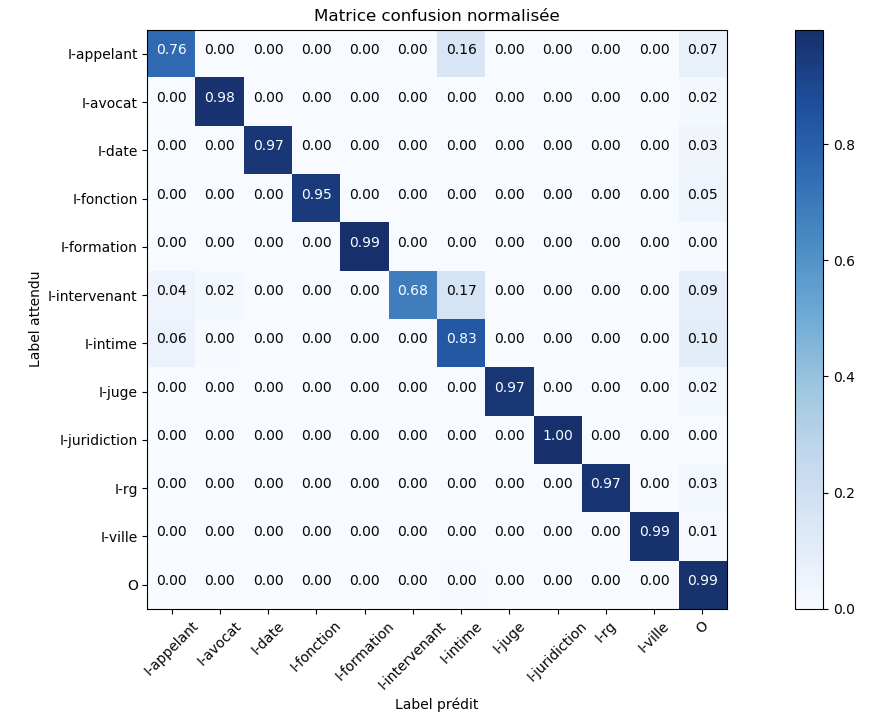
\includegraphics[width=\textwidth]{confusion_matrix_entete.png}
    %\textcolor{red}{Matrices de confusion}
    \caption{Matrice de confusion entre méta-données d'entête avec le modèle CRF}
    \label{fig:structuration:matrice-confusion-entete}
\end{figure}

 De plus, les intervenants apparaissent dans une très faible proportion de documents annotés.  Par ailleurs, une quantité considérable d'\textit{appelants} sont aussi classifiés comme \textit{intimés} (16 \%).  Ce qui signifie que la transition entre la liste des appelants et celle des intimés est difficilement identifiable avec les descripteurs de mots que nous avons définis. La proximité crée aussi des confusions entre les sections CORPS et DISPOSITIF qui se suivent (\figureref{fig:structuration:matrice-confusion-section}). 

\begin{figure}[!htb]
	\centering
	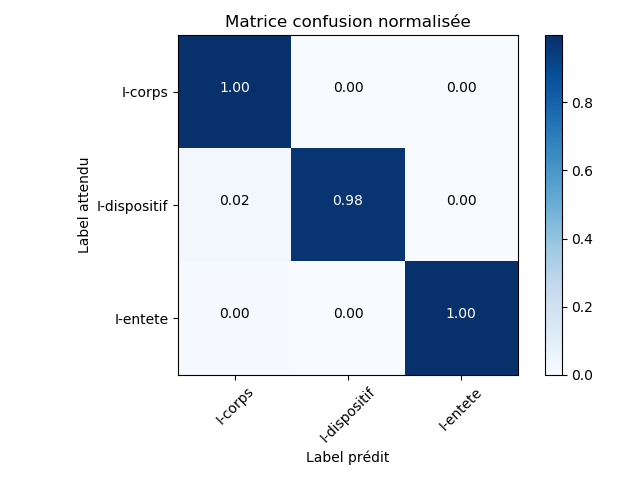
\includegraphics[width=0.6\textwidth]{confusion_matrix_section.png}
	%\textcolor{red}{Matrices de confusion}
	\caption{Matrice de confusion entre lignes des sections avec le modèle CRF}
	\label{fig:structuration:matrice-confusion-section}
\end{figure}

\subsubsection{Redondance des mentions d'entités}
Il est aussi intéressant de remarquer que certaines entités sont répétées dans le document. Par exemple, les noms des parties apparaissent précédemment à une mention qui donne plus de détails. Certaines normes sont aussi citées plusieurs fois et en alternant souvent les formes abrégées et longues (par exemple, la juridiction, la date, les normes). Bien que les différentes occurrences d'une même méta-données ne soient pas toujours identiques, de telles redondances aident à réduire le risque de manquer une entité. Cet aspect peut être exploité afin de combler l'imperfection des modèles.


\subsubsection{Impact de la quantité d'exemples annotés}

\begin{figure}[!htb]
	\centering
	\begin{subfigure}[ht]{\textwidth}
		\centering
		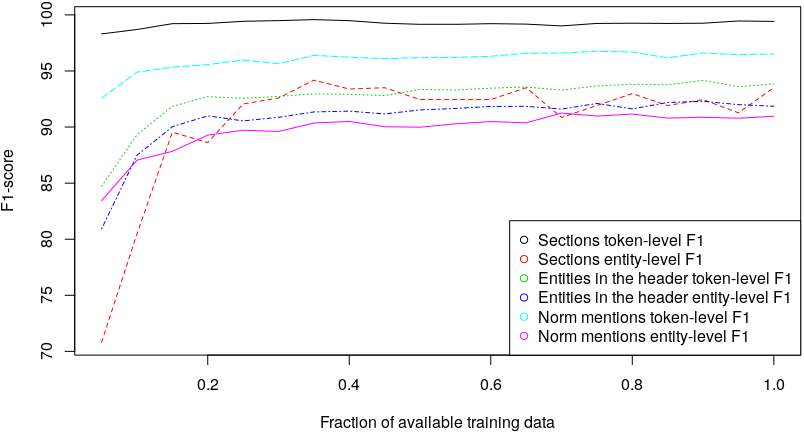
\includegraphics[width=0.9\textwidth]{lc-crf.png} 
		\caption{CRF} \label{fig:structuration:learning-curves-crf}
	\end{subfigure} 
	
	\begin{subfigure}[ht]{\textwidth}
		\centering
		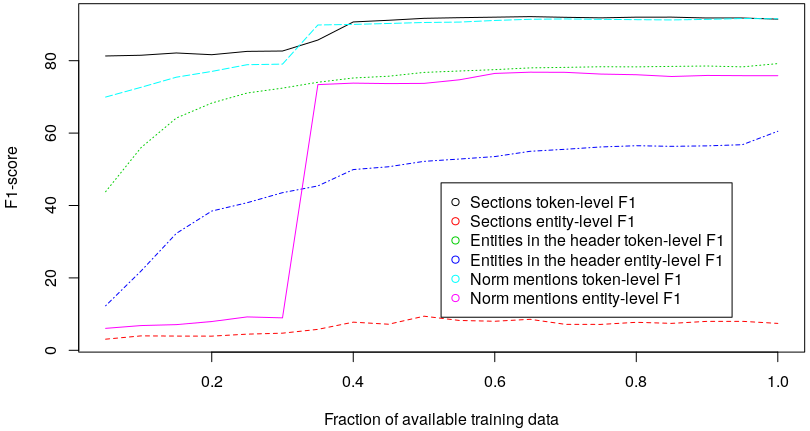
\includegraphics[width=0.9\textwidth]{lc-hmm.png}
		\caption{HMM} \label{fig:structuration:learning-curves-hmm}
	\end{subfigure}
	\caption{Évolution du score F1 en fonction de l'augmentation du nombre de données d'entraînement.} \label{fig:structuration:learning-curves}
\end{figure}

Des expérimentations ont été menées pour évaluer les variations des modèles lorsque l'on augmente le nombre de données d'entraînement. Pour cela, nous avons évalué différentes tailles de la base d'entraînement. Les données ont été divisées en $75\%-25\%$ pour resp. l'entraînement et le test. 20 fractions de l'ensemble d'entraînement ont été utilisées  (de 5\% à 100\%). A chaque session entraînement-test, le même jeu de test a été employé pour les différentes fractions de l'ensemble d'entraînement. Les courbes d'apprentissage des modèles CRF et HMM sont représentées resp. sur les Figures \ref{fig:structuration:learning-curves-crf} (Page \pageref{fig:structuration:learning-curves-crf}) et \ref{fig:structuration:learning-curves-hmm} (Page \pageref{fig:structuration:learning-curves-hmm}) . 



Il apparaît que les scores $F_1$ croissent avec le nombre de données d'entraînement pour les CRF et HMM, mais cette amélioration devient très faible au-delà de 60\% de données d'entraînement quelle que soit la tâche. Il est possible que les exemples ajoutés par la suite partagent la même structure que celle de ceux qui ont été ajoutés auparavant. Ainsi, cette étude doit être étendue à la sélection des exemples les plus utiles. \citet{raman2003exampleSelection} ont démontré les avantages des algorithmes de sélection d'exemples combinés à celle des caractéristiques pour la classification. Les mêmes méthodes sont probablement applicables à l'étiquetage de séquences.



\subsubsection{Descripteurs manuels vs. réseau de neurones}

\begin{table}[!ht]
	\footnotesize
	\centering
	\begin{tabular}{|l|l|l|l|l|l|l|}
		\hline
		&               \multicolumn{3}{c}{\textbf{CRF + descripteurs manuels}} & \multicolumn{3}{|c|}{\textbf{BiLSTM-CRF}}   \\ \cline{2-7}
		& \textit{Precision} & \textit{Rappel}                     & $F_1$ & \textit{Precision} & \textit{Rappel}      & $F_1$ \\ \hline
		\textbf{appelant}      & 82.49              & 69.42                               & 74.72       & 80.26              & 71.53                & 75.04       \\ 
		\textbf{avocat}        & 90.15              & 89.02                               & 89.56       & 84.93              & 87.88                & 86.36       \\ 
		\textbf{date}          & 95.34              & 91.46                               & 93.12       & 95.04              & 90.79                & 92.63       \\ 
		\textbf{fonction}      & 95.87              & 95.08                               & 95.44       & 92.69              & 93.48                & 93.03       \\ 
		\textbf{formation}     & 96.91              & 91.31                               & 93.7        & 91.05              & 89.47                & 89.84       \\ 
		\textbf{intervenant}   & 51.42              & 32.71                               & 36.8        & 31.48              & 20                   & 23.11       \\ 
		\textbf{intime}        & 76.01              & 79.15                               & 77.22       & 67.7               & 75.43                & 70.83       \\ 
		\textbf{juge}          & 95.67              & 94.07                               & 94.84       & 95.44              & 95.56                & 95.46       \\ 
		\textbf{juridiction}   & 98.55              & 98.25                               & 98.33       & 97.95              & 99.22                & 98.57       \\ 
		\textbf{rg}            & 95.46              & 95.29                               & 95.27       & 91.13              & 97.26                & 93.92       \\ 
		\textbf{ville}         & 98.33              & 93.01                               & 94.71       & 91.43              & 95.34                & 93.3        \\ 
		\textbf{norme}         & 91.08              & 90.27                               & 90.67       & 91.43              & 92.65                & 92.03       \\ \hline
		\noalign{\smallskip}\hline\noalign{\smallskip}
		\textbf{Evaluation globale} & 92.2               & 90.09                               & 91.12       & 89.21              & 90.43                & 89.81       \\ \hline
	\end{tabular}
	\caption{Comparaison entre le CRF avec des descripteurs définis manuellement et le BiLSTM-CRF au niveau entité.}\label{tab:structuration:perf-bilstmcrf}
\end{table}

L'ingénierie manuelle des caractéristiques est difficile car arbitraire. Nous avons comparé les performances de nos descripteurs avec celles des réseaux de neurones qui apprennent une représentation des segments. Pour cela nous avons choisi le BiLSTM-CRF de \citet{lample2016nnner} qui fait partie des meilleures approches récentes. La comparaison a été effectuée pour la détection des entités avec le schéma d'étiquetage BIEO et une validation croisée à 9 itérations. Le BiLSTM-CRF prend en entrée les plongements sémantiques Word2Vec \citep{mikolov2013word2vec} des mots. Pour cela, nous avons entraîné des vecteurs de mots à partir d'un corpus jurisprudentiel de plus de 800K documents provenant de \url{www.legifrance.gouv.fr} avec l'implémentation\footnote{\url{https://code.google.com/archive/p/word2vec/}} de \citet{mikolov2013word2vec}. Les vecteurs obtenus ont une dimension de 300. Etant donné que les décisions sont des documents particulièrement longs, leur contenu a été découpé en des morceaux de texte dont la taille n'excède pas 300 mots. Les résultats obtenus par le BiLSTM-CRF sont assez proches de ceux que nous observons avec les descripteurs manuellement définis (\tableref{tab:structuration:perf-bilstmcrf}). Etant donné que ces derniers permettent de mieux détecter certaines entités comme les \textit{intervenants}, les \textit{avocats} ou les numéro \textit{R.G.}, et vice-versa pour les \textit{normes} ou les \textit{appelants} chez le BiLSTM-CRF, une combinaison des deux types de descripteurs pourrait améliorer les résultats actuels. %On peut par exemple exploiter des modèles thématiques déduits en partitionnant (\textit{clustering}) l'ensemble des vecteurs de mots  et les utiliser comme descripteurs définis manuellement. 
 
\subsubsection{Sectionnement en 4 sections pour l'extraction des demandes}
\label{sec:structuration:sectionnement-en-4}

\begin{table}[!htb]
	\footnotesize
	\centering
	\begin{tabular}{|l|c|c|c|}
		\hline
		\multirow{2}{*}{}	&      \multicolumn{3}{|c|}{\textbf{CRF (\%)}}          \\ \cline{2-4} & \textit{Precision} & \textit{Rappel} & $F_1$ \\ \hline
		\textbf{entete} &   99.80 &	99.54 &	99.67      \\ 
		\textbf{litige}      &  96.10 &	97.66	& 96.87       \\ 
		\textbf{motifs}      &   97.31	&95.96	&96.62 \\
		\textbf{dispositif}    &   99.00&	98.49&	98.72  \\ \hline
		\textbf{Evaluation globale} &97.55	&97.55	&97.55       \\ \hline
	\end{tabular}
	\caption{Evaluation au niveau atomique de la détection de 4 sections à l'aide du CRF.} \label{tab:structuration:5folccvCRF-4sections}
\end{table}

Le sectionnement peut permettre de mieux localiser les informations selon leur nature. Pour l'extraction des demandes nous avons dû passer d'un sectionnement à 3 sections comme étudié depuis le début de ce chapitre, vers un sectionnement à 4 sections (cf. Annexe \ref{appendix:exemple-decision} Page \pageref{appendix:exemple-decision}). En effet, la section Corps est remplacé par les deux sections qu'elle englobait: l'exposé du litige (Litige) et les motivations des juges (Motifs). Comme nous le faisons remarquer dans le chapitre \ref{chap:quanta}, les demandes sont généralement énoncées dans la section Litige et les résultats dans le Dispositif. En expérimentant cet affinement du sectionnement par 5-\textit{fold} validation croisée avec les mêmes documents annotés manuellement, les mêmes descripteurs caractéristiques de lignes, le schéma d'étiquetage IO, et le modèle CRF, nous observons les résultats du \tableref{tab:structuration:5folccvCRF-4sections} au niveau atomique. L'Entête reste aisément détectable ($F_1$-mesure=99.67\%) contrairement aux autres sections qui ont quasiment 3\% en moins en moyenne de $F_1$-mesures par rapport à l'entête.


\section{Conclusion}
\label{sec:structuration:conclusion}
L'application des modèles HMM et CRF dans le but de détecter des sections et des entités dans les décisions de justice est une tâche difficile. Ce chapitre a examiné les effets de divers aspects de la conception sur la qualité des résultats. En résumé, malgré une importante réduction du nombre de descripteurs, l'amélioration des résultats semble être insignifiante lorsque l'on sélectionne séparément la représentation du segment et le sous-ensemble de caractéristiques. Cependant, opter pour la bonne configuration en évaluant les approches de sélection combinées avec diverses représentations de segment pourrait peut-être offrir de meilleurs résultats. En raison de la longue durée de recherche du sous-ensemble optimal de descripteurs, il serait préférable d'utiliser un algorithme de sélection beaucoup plus rapide que les méthodes BDS et SFFS que nous avons expérimentées. De plus, même si les résultats s'améliorent avec l'augmentation de la taille de l'échantillon d'apprentissage, la mesure globale $F_1$ semble atteindre une limite très rapidement. Étant donné que certaines entités ne sont pas très bien détectées, il peut être avantageux d'ajouter des exemples appropriés afin de traiter ces problèmes spécifiques.

L'application des modèles pose deux difficultés majeures : l'annotation d'un nombre suffisant d'exemples et la définition de caractéristiques discriminantes. Les efforts d'annotation peuvent être réduits avec un système automatique à faible performance d'étiquetage. Il suffirait alors de vérifier manuellement ces annotations afin de corriger les erreurs commises par le système sur de nouvelles décisions à l'aide d'un outil d'aide à l'annotation. En ce qui concerne la définition des caractéristiques, dans la mesure où notre approche actuelle est réalisée manuellement par l'analyse de quelques documents, il est possible que de tels descripteurs ne s'adaptent pas parfaitement à un nouvel ensemble de données (différents pays, différentes langues, différentes juridictions). Pour éviter les énormes efforts requis pour définir les fonctionnalités manuellement, il serait préférable d'utiliser des descripteurs appris automatiquement à partir de corpus étiquetés ou non, comme des mots incorporés.

Il serait intéressant de poursuivre les travaux proposés sur la tâche de reconnaissance d'entités nommées. L'étude de modèles couplant les approches à descripteurs définis manuellement (e.g., CRF), avec des approches sans définition manuelle (de type apprentissage profond e.g., BiLSTM CRF) semble particulièrement intéressante. Une étude comparative approfondie des limitations des deux approches serait alors souhaitable. Bien que les approches à base d'apprentissage profond apparaissent (légèrement) moins performantes dans nos tests, l'étude de ces approches prometteuse est bien entendu à recommander. Des travaux sur l'impact des techniques de plongement lexical sur la performance de ces systèmes méritent notamment d'être menées.

Pour l'indexation des décisions dans une base de connaissances, il est aussi important de définir des méthodes de désambiguïsation et de résolution pour les entités à occurrences multiples, en plus de la correspondance des entités extraites avec des entités de référence, comme l'ont expérimenté \citet{dozier2010legalnerr} et \citet{cardellino2017legalNERCL}. Ces travaux peuvent être poursuivis par d'autres applications telles que l'anonymisation automatique qui aiderait à publier plus rapidement l'énorme volume de décisions prononcées régulièrement.